\documentclass[a4paper,11pt,fleqn,dvipsnames,oneside,openright]{memoir} 	% Openright aabner kapitler paa hoejresider (openany begge)

%%%% PACKAGES %%%%

% ¤¤ Oversaettelse og tegnsaetning ¤¤ %
\usepackage[utf8]{inputenc}					% Input-indkodning af tegnsaet (UTF8)
\usepackage[danish]{babel}					% Dokumentets sprog
\usepackage[T1]{fontenc}					% Output-indkodning af tegnsaet (T1)
\usepackage{ragged2e,anyfontsize}			% Justering af elementer
\usepackage{fixltx2e}						% Retter forskellige fejl i LaTeX-kernen
																			
% ¤¤ Figurer og tabeller (floats) ¤¤ %
\usepackage{graphicx} 						% Haandtering af eksterne billeder (JPG, PNG, EPS, PDF)

\usepackage{subfig}

%\usepackage{eso-pic}						% Tilfoej billedekommandoer paa hver side
%\usepackage{wrapfig}						% Indsaettelse af figurer omsvoebt af tekst. \begin{wrapfigure}{Placering}{Stoerrelse}
\usepackage[space]{grffile}					% Bør gøre det muligt at have mellemrum i filnavne.
\usepackage{multirow}                		% Fletning af raekker og kolonner (\multicolumn og \multirow)
\usepackage{multicol}         	        	% Muliggoer output i spalter
\usepackage{rotating}						% Rotation af tekst med \begin{sideways}...\end{sideways}
\usepackage{colortbl} 						% Farver i tabeller (fx \columncolor og \rowcolor)
\usepackage[usenames,dvipsnames]{xcolor}	% Definer farver med \definecolor. Se mere: http://en.wikibooks.org/wiki/LaTeX/Colors
%\usepackage{flafter}						% Soerger for at floats ikke optraeder i teksten foer deres reference
\let\newfloat\relax 						% Justering mellem float-pakken og memoir
\usepackage{float}							% Muliggoer eksakt placering af floats, f.eks. \begin{figure}[H]
\setlength{\heavyrulewidth}{0.15em}			% Sætter \toprule og \bottomrule til fast størrelse (0.08 er default)
%\setlength{\lightrulewidth}{0.05em}		% Sætter \midrule til fast størrelse (0.05 er default)
\usepackage{array}							% Bruges i forbindelse med \newcolumntype-command under egne commands
\usepackage{pdfpages}						% Bruges så der kan indsættes pdf, som sider (forside for eksempel)
\usepackage{wrapfig}
\usepackage[section]{placeins}				% Indsætter en border så billeder bliver placeret inden for den section de er indsat
\usepackage{lastpage}						% Anvendes til at se total antal sider

% ¤¤ Matematik mm. ¤¤
\usepackage{amsmath,amssymb,stmaryrd} 		% Avancerede matematik-udvidelser
\usepackage{mathtools}						% Andre matematik- og tegnudvidelser
\usepackage{textcomp}                 		% Symbol-udvidelser (f.eks. promille-tegn med \textperthousand )
\usepackage{rsphrase}						% Kemi-pakke til RS-saetninger, f.eks. \rsphrase{R1}
\usepackage[version=3]{mhchem} 				% Kemi-pakke til flot og let notation af formler, f.eks. \ce{Fe2O3}
\usepackage{siunitx}						% Flot og konsistent praesentation af tal og enheder med \si{enhed} og \SI{tal}{enhed}
\sisetup{locale=DE}							% Opsaetning af \SI (DE for komma som decimalseparator) 

% ¤¤ Referencer og kilder ¤¤ %
\usepackage[danish]{varioref}				% Muliggoer bl.a. krydshenvisninger med sidetal (\vref)
\usepackage{natbib}							% Udvidelse med naturvidenskabelige citationsmodeller
\usepackage{xr-hyper}							% Referencer til eksternt dokument med \externaldocument{<NAVN>}
\externaldocument[DokRap-]{../Dokumentationsrapport/Dokumentationsrapport}	% Muliggør eksterne referencer til dokumentationsrapporten
%\usepackage{glossaries}					% Terminologi- eller symbolliste (se mere i Daleifs Latex-bog)



% ¤¤ Misc. ¤¤ %
\usepackage{lipsum}							% Dummy text \lipsum[..]
\usepackage[shortlabels]{enumitem}			% Muliggoer enkelt konfiguration af lister
\usepackage{pdfpages}						% Goer det muligt at inkludere pdf-dokumenter med kommandoen \includepdf[pages={x-y}]{fil.pdf}	
\pdfoptionpdfminorversion=6					% Muliggoer inkludering af pdf dokumenter, af version 1.6 og hoejere
\pretolerance=2500 							% Justering af afstand mellem ord (hoejt tal, mindre orddeling og mere luft mellem ord)

% Kommentarer og rettelser med \fxnote. Med 'final' i stedet for 'draft' udloeser hver note en error i den faerdige rapport.
\usepackage[footnote,draft,danish,silent,nomargin]{fixme}	

%lists
\usepackage{listings}	


%%%% CUSTOM SETTINGS %%%%

% ¤¤ Marginer ¤¤ %
\setlrmarginsandblock{3.5cm}{2.5cm}{*}		% \setlrmarginsandblock{Indbinding}{Kant}{Ratio}
\setulmarginsandblock{2.5cm}{3.0cm}{*}		% \setulmarginsandblock{Top}{Bund}{Ratio}
\checkandfixthelayout 						% Oversaetter vaerdier til brug for andre pakker

%	¤¤ Afsnitsformatering ¤¤ %
\setlength{\parindent}{0mm}           		% Stoerrelse af indryk
\setlength{\parskip}{3mm}          			% Afstand mellem afsnit ved brug af double Enter
\linespread{1,1}							% Linie afstand
\newcommand{\tab}{\hspace*{2em}}			% ved \tab{} indrykkes det i klammerne ind
\usepackage{titlesec}							%Muliiggøre ændring af sections i alle lag
\titleformat*{\section}{\LARGE\bfseries\color{NavyBlue}}		%section = størst
\titleformat*{\subsection}{\Large\bfseries\color{RoyalBlue}}		%sub og subsub har samme størrelse
\titleformat*{\subsubsection}{\Large\bfseries}
\titleformat*{\paragraph}{\large\bfseries}		%Benyttes umiddelbart ikke
\titleformat*{\subparagraph}{\large\bfseries}	%Benyttes umiddelbart ikke

% ¤¤ Litteraturlisten ¤¤ %
\bibpunct[,]{[}{]}{;}{a}{,}{,} 				% Definerer de 6 parametre ved Harvard henvisning (bl.a. parantestype og seperatortegn)
\bibliographystyle{bibtex/harvard}			% Udseende af litteraturlisten.

% ¤¤ Indholdsfortegnelse ¤¤ %
\setsecnumdepth{subsubsection}		 		% Dybden af nummerede overkrifter (part/chapter/section/subsection)
\maxsecnumdepth{subsection}					% Dokumentklassens graense for nummereringsdybde
\settocdepth{subsubsection} 				% Dybden af indholdsfortegnelsen

% ¤¤ Lister ¤¤ %
\setlist{
  topsep=-5pt,								% Vertikal afstand mellem tekst og listen	Default: 0
  itemsep=-1ex,								% Vertikal afstand mellem items
} 

% ¤¤ Visuelle referencer ¤¤ %
\usepackage[colorlinks]{hyperref}			% Danner klikbare referencer (hyperlinks) i dokumentet.
\hypersetup{colorlinks = true,				% Opsaetning af farvede hyperlinks (interne links, citeringer og URL)
    linkcolor = black,
    citecolor = black,
    urlcolor = black
}

% ¤¤ Opsaetning af figur- og tabeltekst ¤¤ %
\usepackage{caption}
\captionnamefont{\small\bfseries\itshape}	% Opsaetning af tekstdelen ('Figur' eller 'Tabel')
\captiontitlefont{\small}					% Opsaetning af nummerering
\captiondelim{. }							% Seperator mellem nummerering og figurtekst
\hangcaption								% Venstrejusterer flere-liniers figurtekst under hinanden
\captionsetup{width=\linewidth,labelfont={bf,it}}
\setlength{\abovecaptionskip}{5pt}			% Afstand over figurteksten
\setlength{\belowcaptionskip}{-12pt}		% Afstand under figurteksten
		
% ¤¤ Navngivning ¤¤ %
\addto\captionsdanish{
	\renewcommand\appendixname{Appendiks}
	\renewcommand\contentsname{Indholdsfortegnelse}	
	\renewcommand\appendixpagename{Appendiks}
	\renewcommand\appendixtocname{Appendiks}
	\renewcommand\cftchaptername{\chaptername~}				% Skriver "Kapitel" foran kapitlerne i indholdsfortegnelsen
	\renewcommand\cftappendixname{\appendixname~}			% Skriver "Appendiks" foran appendiks i indholdsfortegnelsen
}

% ¤¤ Kapiteludssende ¤¤ %
\definecolor{chapnumcolor}{RGB}{23,54,93}		% Definerer en farve til brug til kapiteludseende
\definecolor{chapfontcolor}{RGB}{29,69,118}
\newif\ifchapternonum

\makechapterstyle{jenor}{					% Definerer kapiteludseende frem til ...
  \renewcommand\beforechapskip{0pt}
  \renewcommand\printchaptername{}
  \renewcommand\printchapternum{}
  \renewcommand\printchapternonum{\chapternonumtrue}
  \renewcommand\chaptitlefont{\fontfamily{pbk}\fontseries{db}\fontshape{n}\fontsize{25}{35}\selectfont\raggedleft\color{chapfontcolor}}
  \renewcommand\chapnumfont{\fontfamily{pbk}\fontseries{m}\fontshape{n}\fontsize{1in}{0in}\selectfont\color{chapnumcolor}}
  \renewcommand\printchaptertitle[1]{%
    \noindent
    \ifchapternonum
    \begin{tabularx}{\textwidth}{X}
    {\let\\\newline\chaptitlefont ##1\par} 
    \end{tabularx}
    \par\vskip-2.5mm\hrule
    \else
    \begin{tabularx}{\textwidth}{Xl}
    {\parbox[b]{\linewidth}{\chaptitlefont ##1}} & \raisebox{-15pt}{\chapnumfont \thechapter}
    \end{tabularx}
    \par\vskip2mm\hrule
    \fi
  }
}											% ... her

\chapterstyle{jenor}						% Valg af kapiteludseende - Google 'memoir chapter styles' for alternativer

% ¤¤ Sidehoved ¤¤ %

\makepagestyle{AAU}							% Definerer sidehoved og sidefod udseende frem til ...
\makepsmarks{AAU}{%
	\createmark{chapter}{left}{shownumber}{}{. \ }
	\createmark{section}{right}{shownumber}{}{. \ }
	\createplainmark{toc}{both}{\contentsname}
	\createplainmark{lof}{both}{\listfigurename}
	\createplainmark{lot}{both}{\listtablename}
	\createplainmark{bib}{both}{\bibname}
	\createplainmark{index}{both}{\indexname}
	\createplainmark{glossary}{both}{\glossaryname}
}
\nouppercaseheads											% Ingen Caps oenskes

\makeevenhead{AAU}{Test}{}{\leftmark}					% Definerer lige siders sidehoved (\makeevenhead{Navn}{Venstre}{Center}{Hoejre})
\makeoddhead{AAU}{\rightmark}{}{Ingeniørhøjskolen, Aarhus Universitet}		% Definerer ulige siders sidehoved (\makeoddhead{Navn}{Venstre}{Center}{Hoejre})
\makeevenfoot{AAU}{\thepage}{}{}							% Definerer lige siders sidefod (\makeevenfoot{Navn}{Venstre}{Center}{Hoejre})
\makeoddfoot{AAU}{}{}{\thepage}								% Definerer ulige siders sidefod (\makeoddfoot{Navn}{Venstre}{Center}{Hoejre})
\makeheadrule{AAU}{\textwidth}{0.5pt}						% Tilfoejer en streg under sidehovedets indhold
\makefootrule{AAU}{\textwidth}{0.5pt}{1mm}					% Tilfoejer en streg under sidefodens indhold

\copypagestyle{AAUchap}{AAU}								% Sidehoved for kapitelsider defineres som standardsider, men med blank sidehoved
\makeoddhead{AAUchap}{}{}{}
\makeevenhead{AAUchap}{}{}{}
\makeheadrule{AAUchap}{\textwidth}{0pt}
\aliaspagestyle{chapter}{AAUchap}							% Den ny style vaelges til at gaelde for chapters
															% ... her
															
\pagestyle{AAU}												% Valg af sidehoved og sidefod



% Opsætning af source code import
% \lstinputlisting{sti../navn.endelse}
\lstset{
  language=C,                		% choose the language of the code
  numbers=left,                   	% where to put the line-numbers
  stepnumber=1,                   	% the step between two line-numbers.        
  numbersep=5pt,                  	% how far the line-numbers are from the code
  backgroundcolor=\color{white},  	% choose the background color. You must add \usepackage{color}
  showspaces=false,               	% show spaces adding particular underscores
  showstringspaces=false,         	% underline spaces within strings
  showtabs=false,                 	% show tabs within strings adding particular underscores
  tabsize=2,                      	% sets default tabsize to 2 spaces
  captionpos=b,                   	% sets the caption-position to bottom
  breaklines=true,                	% sets automatic line breaking
  breakatwhitespace=true,         	% sets if automatic breaks should only happen at whitespace
  title=\lstname,                 	% show the filename of files included with \lstinputlisting;
  emph={ uint8, uint16, void }, emphstyle={\color{blue}}	% tilføj variabel hvis de skal markeres blå
}






%%%% CUSTOM COMMANDS %%%%

% ¤¤ Billede hack ¤¤ %
\newcommand{\figur}[4]{
		\begin{figure}[H] \centering
			\includegraphics[width=#1\textwidth]{Billeder/#2}
			\caption{#3}\label{#4}
		\end{figure} 
}


% ¤¤ Venstre orienterer al tekst i p{Ycm} ¤¤ %
\newcolumntype{x}[1]{%
>{\raggedright\hspace{0pt}}p{#1}}

% ¤¤ Newline til x{} ¤¤ %
% \\ virker åbenbart ikke når man selv laver en columntype... :(
\newcommand{\tn}{\tabularnewline}

% ¤¤ Newline til x{} ¤¤ %
% \\ virker åbenbart ikke når man selv laver en columntype... :(
\newcommand{\tnhl}{\tabularnewline\hline}



% ¤¤ Nyt environment til indsættelse af A3-størrelse figurer
\newenvironment{A3Figure}
{
	\cleardoublepage
	\pageaiii
	\setlength{\pdfpagewidth}{\paperheight} % Change the pdf page to A3 height
	\setlength{\pdfpageheight}{\paperwidth} % Change the pdf height to A3 width
	\setlength{\textwidth}{\paperheight - \the\spinemargin-\the\foremargin} % Change the textwidth
}
{
	\cleardoublepage	
}

% funktions beskrivelse void argument%
\newcommand{\funcDescrip}[2]{
\textbf{{\color{blue} #1} #2({\color{blue} void})} \\
}

% funktions beskrivelse 1 argument%
\newcommand{\funcDescripOne}[4]{
\textbf{{\color{blue} #1} #2({\color{blue} #3} #4)} \\
}

% funktions beskrivelse 2 argument%
\newcommand{\funcDescripTwo}[6]{
\textbf{{\color{blue} #1} #2({\color{blue} #3} #4, {\color{blue} #5} #6)} \\
}

% opsætning af funktions tabel %
\newcommand{\funcTabel}[4]{
\begin{tabular}{p{0.2cm}p{3cm}p{11cm}} \hline
	&	\textbf{Description:} 		& 	#1	\\
	&	\textbf{Parameters:} 		& 	#2	\\
	&	\textbf{Return Value:}		& 	#3	\\
	&	\textbf{Side Effects:}		&	#4	\\
\end{tabular}
}


% ¤¤ Units i math-environments ¤¤ %
\newcommand{\mathUnit}[2]{\mathrm{\si{#1}{#2}}}







% ¤¤ Pæn opsætning af titelblad-dele ¤¤ %
% ¤¤ Husk at ændre dato i senere projekter ¤¤ %
\newcommand{\titelblad}[2]{
\begin{tabular}[ht]{x{7cm}x{7cm}}
\textbf{Navn: } #1		&\textbf{Studienummer: } #2	\tn
\textbf{Dato} 2013-05-31	\tn
\multicolumn{2}{l}{\textbf{Underskrift: }\line(1,0){340}}
\end{tabular}
}


% ¤¤ Specielle tegn ¤¤ %
\newcommand{\grader}{^{\circ}\text{C}}   % Grader C, virker kun i math-environments
\newcommand{\gr}{^{\circ}}
\newcommand{\g}{\cdot}		% Gange i math-environments
\newcommand{\grC}{$^{\circ}\mathrm{C}$}		% Grader C, uden for math-environments

%%%% ORDDELING %%%%

\hyphenation{}

%%%Indsat af Søren%%%
\usepackage{listings}
\usepackage{color}
 
\definecolor{dkgreen}{rgb}{0,0.6,0}
\definecolor{gray}{rgb}{0.5,0.5,0.5}
\definecolor{mauve}{rgb}{0.58,0,0.82}
 
\lstset{ %
  language=Octave,                % the language of the code
  basicstyle=\footnotesize,           % the size of the fonts that are used for the code
  numbers=left,                   % where to put the line-numbers
  numberstyle=\tiny\color{gray},  % the style that is used for the line-numbers
  stepnumber=2,                   % the step between two line-numbers. If it's 1, each line 
                                  % will be numbered
  numbersep=5pt,                  % how far the line-numbers are from the code
  backgroundcolor=\color{white},      % choose the background color. You must add \usepackage{color}
  showspaces=false,               % show spaces adding particular underscores
  showstringspaces=false,         % underline spaces within strings
  showtabs=false,                 % show tabs within strings adding particular underscores
  frame=single,                   % adds a frame around the code
  rulecolor=\color{black},        % if not set, the frame-color may be changed on line-breaks within not-black text (e.g. comments (green here))
  tabsize=2,                      % sets default tabsize to 2 spaces
  captionpos=b,                   % sets the caption-position to bottom
  breaklines=true,                % sets automatic line breaking
  breakatwhitespace=false,        % sets if automatic breaks should only happen at whitespace
  title=\lstname,                   % show the filename of files included with \lstinputlisting;
                                  % also try caption instead of title
  keywordstyle=\color{blue},          % keyword style
  commentstyle=\color{dkgreen},       % comment style
  stringstyle=\color{mauve},         % string literal style
  escapeinside={\%*}{*)},            % if you want to add LaTeX within your code
  morekeywords={*,...},              % if you want to add more keywords to the set
  deletekeywords={...}              % if you want to delete keywords from the given language
}											% Preamble 
\raggedbottom													% LaTeX "straekker" ikke teksten

%\includeonly{file1,file2}										% Inkluder kun specifikke filer 

\begin{document}												% Starter
\frontmatter													% Forindhold - nummereres med romertal
\thispagestyle{empty}
\begin{flushright}
\vspace{3cm}

\phantom{hul}

\phantom{hul}

\phantom{hul}

\textsl{\Huge Skeleton Project} \\ \vspace{1cm}

\rule{13cm}{3mm} \\ \vspace{1.5cm}
\vspace{1cm}


\includegraphics[width=0.4\textwidth]{4.Construction/pictures/skeleton-cover.jpg}

\vspace{2cm} 
\textsc{\Large Skeleton Project V1 \\
Group of project \\
Faculty\\
Delivery date\\}
\end{flushright}

 %%%%%% Resumé %%%%%%
\chapter{Resumé og Abstract}
\label{chap:resume}


\section*{Abstract}


\section*{Resumé}

Formålet med dette bachelorprojekt er at udvikle en overvågningsdrone der nemt og omkostningsfrit kan overvåge et område. Dronen udvikles for at skabe et alternativ til dyr og ressourcekrævende overvågning udført af mennesker.
Projektet er designet og udviklet på Ingeniørhøjskolen Aarhus Universitet.

I projektet omdannes en fjernstyret quadrocopter til en drone, som skal bruges til overvågning. Ud fra brugers anvisninger skal drone autonomt kunne flyve til GPS positioner og tage overvågningsbilleder.  

Den udviklede drone består af en Aeroquad ARF quadrocopter med påmonteret GPS, højdemåler og mobilt kommunikationsmodul. Systemets bruger indstille droneflyvning samt monitorerer data fra tidligere flyvninger via en webapplikation.  

I projektforløbet lykkedes det at implementere en fuldt fungerende server, samt kommunikationslink og udveksling af data mellem server og drone. Desuden blev opsamling af data fra GPS, kompas og højdemåler fuldt ud implementeret. Det lykkedes endvidere at implementere hovedparten af webapplikationen og dronens autonome flyvning.







%%%% Indholdsfortegnelse (TOC) %%%%
\tableofcontents*												%Indholdsfortegnelsen (kaldet ToC) 

\mainmatter														% Hovedindhold - nummereres fra side 1




\chapter{Systemarkitektur}

\section{Revisionshistorik}
\begin{table}[H]
	\centering
		\begin{tabular}{|p{2 cm}|p{2 cm}|p{3 cm}|p{6 cm}|} 
		\hline
			\textbf{Rev. Nr} & \textbf{Dato}		& \textbf{Initialer} 	& \textbf{Ændring} \\ \hline
			1.0 	& & &  \\ \hline
			1.1 	& & &	\\ \hline
		\end{tabular}
	\caption{Revisionshistorik}
	%\label{tab:TC1}
\end{table}

\vspace{1.5cm}

\section{Ordforklaring}
\begin{table}[H]
	\centering
		\begin{tabular}{|p{2.5cm}|p{4.5 cm}|p{6.5 cm}|} 
		\hline
			\textbf{Forkortelse} & \textbf{Betydning} & \textbf{Forklaring} \\ \hline
			 &  &  \\ \hline
			 &  & \\ \hline
		\end{tabular}
	\caption{Ordforklaring}
	%\label{tab:TC1}
\end{table}

\vspace{2cm}

\section{Indledning}
Dette kapitel beskriver hvilke enheder systemet består af samt grænseflader mellem
enhederne. Til at beskrive hardware og tilhørende grænseflader benyttes SysML diagrammer, mens software og tilhørende grænseflader beskrives med UML diagrammer.

\chapter{Forord}

Dette projekt blev tilbudt som et bachelorprojekt af Ingeniørhøjskolen Aarhus Universitet. Grundet tidens stigende fokus på droner ønskede Ingeniørhøjskolen det undersøgt hvorvidt det var muligt at udvikle en drone.

Der var i udgangspunkt ingen begrænsninger for hvad bachelorprojektet kunne eller skulle indeholde. Derfor har gruppen på egen hånd opsat krav, designet og udformet bachelorprojektet \textit{Autonom overvågningsdrone}.
 
Projekt, projektrapport og tilhørende dokumentationen er udarbejdet af projektgruppe 14123, bestående af 3 ingeniørstuderende. Gruppen er blevet bevilliget økonomisk støtte til indkøb af drone, sensorer og andet hardware. Ydermere har gruppen fået vejledning og rådgivning af en vejleder tilknyttet fra Ingeniørhøjskolen Aarhus Universitet.  \\


\subsection*{\textit{Referencer} \vspace{-0.3cm}}
Betegnelsen [x] hentyder til en reference, som står i referencelisten sidst i rapporten. 
%%%%%% Indledning %%%%%%
\chapter{Indledning}
\label{chap:indledning}

I den moderne verden findes der mange forskellige former for overvågning, og overvågning foregår overalt. Primært bruges overvågning til at skabe tryghed og forebygge mod kriminalitet, hvilket de fleste mennesker er positivt stemt overfor. Men pga. en stigning i brugen af overvågning, bruges der gradvist flere og flere ressourcer på området. 
I projektet undersøges det, hvorvidt det er muligt at udvikle en autonom overvågningsdrone. Det er gruppens mål at udvikle en drone der ud fra administrators anvisninger kan overvåge og tage billeder af et defineret område. Dronen udvikles for at mindske mængden af menneskelige ressourcer der bruges på overvågning.

Formålet med projektet er at konstruere en drone, som autonomt kan overvåge et givet område. Dronen gøres i stand til at kommunikere med en server, samt orientere sig om egen GPS position, flyvehøjde og flyveretning. Gennem kommunikation med server henter dronen flyveopsætning og flyver på egen hånd ud og overvåger et defineret område.
Projektet er planlagt, designet og konstrueret hen over en periode på 4 måneder.

Projektrapporten er sat op efter en standard, hvor systemet indledningsvis beskrives på et abstrakt niveau. Herefter beskrives krav til produktet, og der gåes mere analytisk og teknisk til værks. Rapporten afsluttes af med resultater, diskussion af resultater samt en konklusion.



%%%%%% Opgaveformulering %%%%%%
\chapter{Opgaveformulering}
\label{chap:opgaveformulering}

Hovedformålet med projektet er at udvikle en drone, der autonomt kan overvåge et område. Overvågningen skal foregå fra luften, hvor dronen flyver mellem forskellige GPS positioner som den overvåger og tager billeder af. Området som drone skal overvåge indstilles af systemets bruger via en webapplikation.


\chapter{Systembeskrivelse}
\vspace{-1cm}
På Ingeniørhøjskolen Aarhus Universitet forefindes en AeroQuad ARF Quadrocopter. 
Målet med projektet er at omdanne quadrocopteren til en autonom overvågningsdrone.

Dronen skal ud fra brugers anvisninger overvåge og tage billeder af et defineret område. 
Dronen tilgås via en webapplikation der fungerer som en grafisk brugerflade mellem bruger og systemet.  Via webapplikationen kan bruger oprette flyveopsætninger til drone samt se billeder og flyverute fra tidligere flyvninger.  
Når der laves ny flyveopsætning vælger bruger en række GPS positioner som dronen skal flyve til, flyvehøjde og hvorvidt der skal tages billeder ved de valgte GPS positioner. Når bruger har lavet en ny flyveopsætning, stilles flyveopsætningen tilgængelig for dronen på server.  

Da dronen skal flyve autonomt, er det vigtigt den kan orientere sig på egen hånd. Derfor er dronen udstyret med GPS, afstands sensorer og kompas.
Til enhver tid, skal kommunikation mellem drone og server foregå via mobilt netværk. Der gøres hovedsageligt brug af 3G netværket, men i områder med dårlig forbindelse vil der blive gjort brug af 2G som fall-back netværk. 

\vspace{-0.5cm}

\section*{Systemskitse}
\vspace{-0.5cm}
Bruger benytter en computer til at tilgå webapplikation og lave en ny flyveopsætning. Når bruger har lavet en ny flyveopsætning, overføres flyveopsætningen via internettet til server, hvor den gøres tilgængelig for dronen.
 
Via det mobile 3G netværk kommunikerer drone med server. 
Inden flyvning påbegyndes henter drone flyveopsætning fra server og under flyvning sender dronen information om nuværende GPS position og overfører billeder til server. 
Under flyvning kontrollerer drone løbende egen GPS position via kommunikation med GPS satellitter. Dette gør den for at opdatere egen position og for efterfølgende at kunne beregne den korrekte flyveorientering. 



\vspace{-5pt}
%Systemskitse
\begin{figure}[H]
\centering
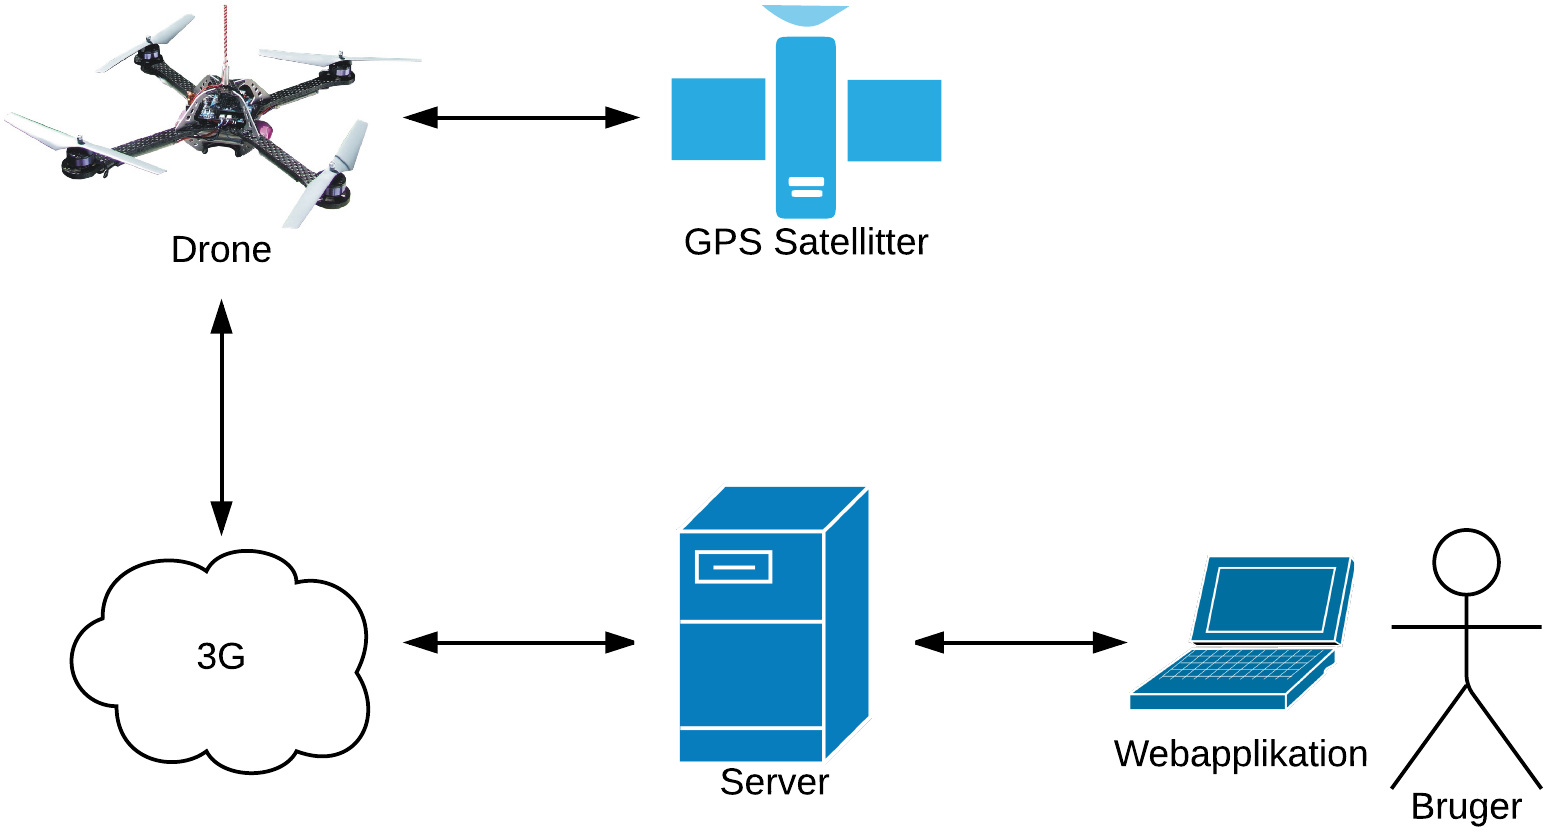
\includegraphics[width=1\textwidth]{Billeder/Projektbeskrivelse.png}
\vspace{-.5cm}
\caption{Systemskitse}
\label{fig:Systemskitse}
\end{figure}
%%%%%% Krav %%%%%%
\chapter{Krav}
\vspace{-0.5cm}
I dette afsnit beskrives kravene til projektet [1]. Indledningsvis præsenteres funktionelle krav  ved brug af use cases. På figur \ref{fig:useCaseDiagram} vises et use diagram, der viser aktører og use cases tilhørende systemet. Efter use case diagrammet følger en kort beskrivelse af de seks use cases og deres funktion. Afsnittet afsluttets med ikke-funktionelle krav, der er både er krav til systemet som helhed og til systemets blokke.
\vspace{-0.3cm}

\section{Funktionelle krav}
\vspace{-0.2cm}
Til systemet er der identificeret de 2 aktører: Bruger \& GPS-satellitter. Bruger er primær aktør der ønsker at initialisere og styre systemet. Bruger er ansvarlig for at oprette flyveopsætninger på webapplikationen og tilslutte batteri til dronen.
GPS-satellitter er sekundær aktør, der gør det muligt for dronen at finde egen position. 
På figur \ref{fig:useCaseDiagram} vises et use case diagram, der viser systemets aktørerne og i hvilke use cases aktørerne optræder. 
\begin{figure}[H]
	\centering
	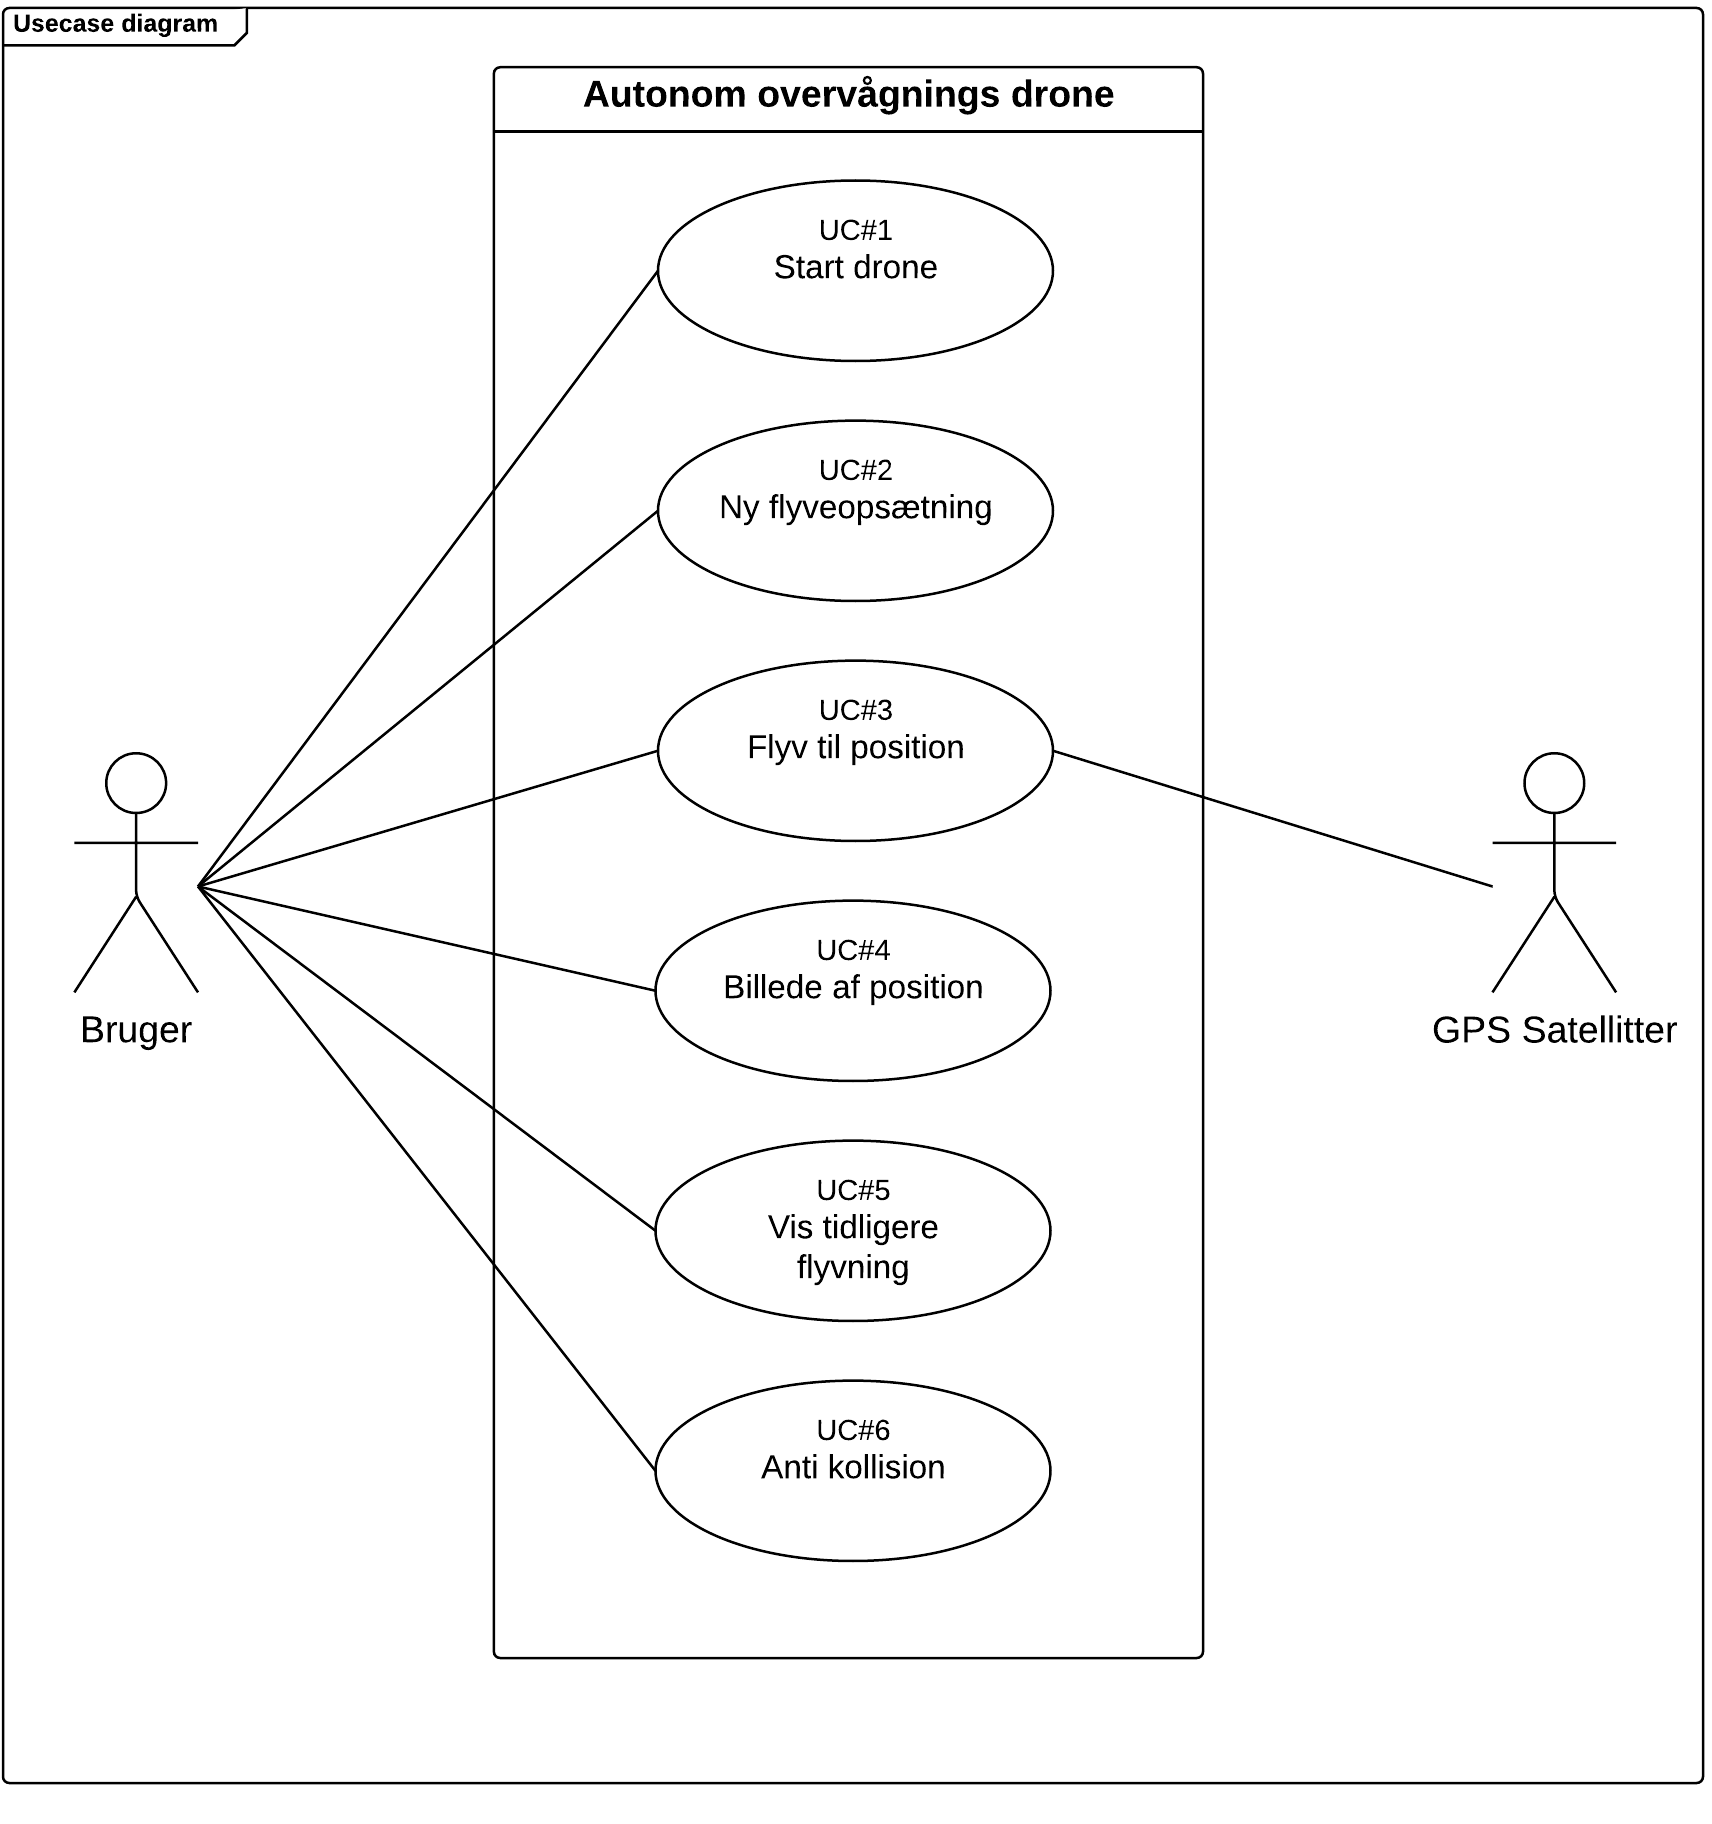
\includegraphics[width=0.75\textwidth]{Billeder/Krav/Use_case_diagram}
	\vspace{-0.3cm}	
	\caption{Use case diagram}
	\label{fig:useCaseDiagram}
\end{figure}

\newpage

I projektets kravspecifikation er alle use cases beskrevet som fully dressed use cases. I fully dressed use cases beskrives hvordan hovedforløb ser ud i en given use case, hvis den succesfuldt gennemføres. Desuden beskrives startbetingelse, aktører og tilføjelser.

Nedenfor beskrives hovedforløb og funktion af de seks use cases:\\

\textbf{Use case 1: Start drone} \\
Bruger tilslutter batteri til drone og dronen initialiseres. Drone sender information om nuværende position til server.\\

\textbf{Use case 2: Ny flyveopsætning} \\
Bruger logger på webapplikation og opretter en ny flyveopsætning. Flyveopsætningen sættes tilgængelig for drone på server.\\

\textbf{Use case 3: Flyv til position}\\
Drone henter flyveopsætning fra server og påbegynder flyvning. Under flyvning tilpasser drone  løbende flyvehøjde og flyveorientering og fortsætter flyvning mod ønsket position. \\

\textbf{Use case 4: Billede af position} \\
Når drone er ankommet til ønsket GPS position tages et billede. Hvis billedet accepteres, flyver dronen videre mod næste GPS koordinat eller til udgangsposition. \\

\textbf{Use case 5: Vis tidligere flyvninger} \\
Bruger tilgår webapplikation for at se flyveruter og billeder tidligere flyvninger.\\

\textbf{Use case 6: Antikollision} \\
Drones antikollisions sensorer bruges til at detekterer forhindringer. I tilfælde af forhindringer ændre drone enten flyveretning eller flyvehøjde for at undgå kollision. \\



\section{Ikke-funktionelle krav}

De ikke-funktionelle krav opstilles ud fra systemspecifikationerne og er krav som ikke kan defineres i use cases. Disse krav har ingen indvirkning på systemets endelig funktion, kun systemspecifikationer.  

De ikke-funktionelle krav opstilles i fem grupper. Nogle krav er generelle krav til systemet, mens andre krav mere specifikt omhandler drone, server og webapplikation eller dataopsamling. 
De ikke-funktionelle krav bruges til at sikre system performance, eksempelvis stilles krav til de hardwaremoduler og sensorer der er monteret på dronen. 

\section{Projektafgrænsning}

Det er blevet vedtaget at implementere systemet som vist på figur ???????.
Der blev fra dag et af besluttet at afgrænse systemets omfang, således at der kunne sættes et realistisk mål i forhold til projekts omfang. \\
Et af afgrænsningerne var videokameraet. Det var tiltænkt at dronen skulle have et videokamera fast monteret, som skulle bruges til at live streame, i samme stil som hvis et stationært overvågningskamera blev anvendt.
Derudover blev der besluttet at nøjes med at bruge lavere kvalitets billeder, for  at gøre upload tiden mindre og derved fokusere på flyvningen.

I kravspecifikationen beskrives det at ethvert device med internet adgang kan benytte webapplikationen. Afhængigt af hvilket device der benytter webapplikationen, kræves en ny opsætning. Derfor er det besluttet kun at designe og implementere webapplikationen til en computer.

Flyvehøjde - bevidst valg af teknologi til højdemåling
Flyvehøjden til tests er bevidst valgt til at være under 5m. Dette skyldes valg af sensorer, da den valgte teknologi der anvendes har en maksimal rækkevidde på 5m. Derudover er højden valgt for at have mere kontrol over dronen under flyvning. 

Projektet blev opdelt i iterationer. Der blev valgt 4 iterationer, hvor den første iteration har den største prioritet, mens den sidste iteration prioriteres mindre højt. Dette medfører at man sikrer at de vigtigste dele af systemet implementeres først. Disse iterationer er beskrevet i projektets dokumentation[x].


%%%%%% Projektbeskrivelse %%%%%%
\section{Projektbeskrivelse}

\section{Systemarkitektur}
\label{chap:systemarkitektur}

Domain modellen anvendes som en overgang mellem kravspecifikation og systemarkitektur.
I kravspecifikation beskrives hvad der sker ved interaktion med systemet. Mens
systemarkitekturen bruges til at beskrive systemet i blokke og til at skitsere både interne
og eksterne forbindelser. Domain modellen bruges til at beskrive hele systemets domæne.
Der kigges ikke på hardware vs. software, der kigges i stedet på "enheder"og deres
ansvarsområder.\\

\begin{figure}[H]
	\centering
	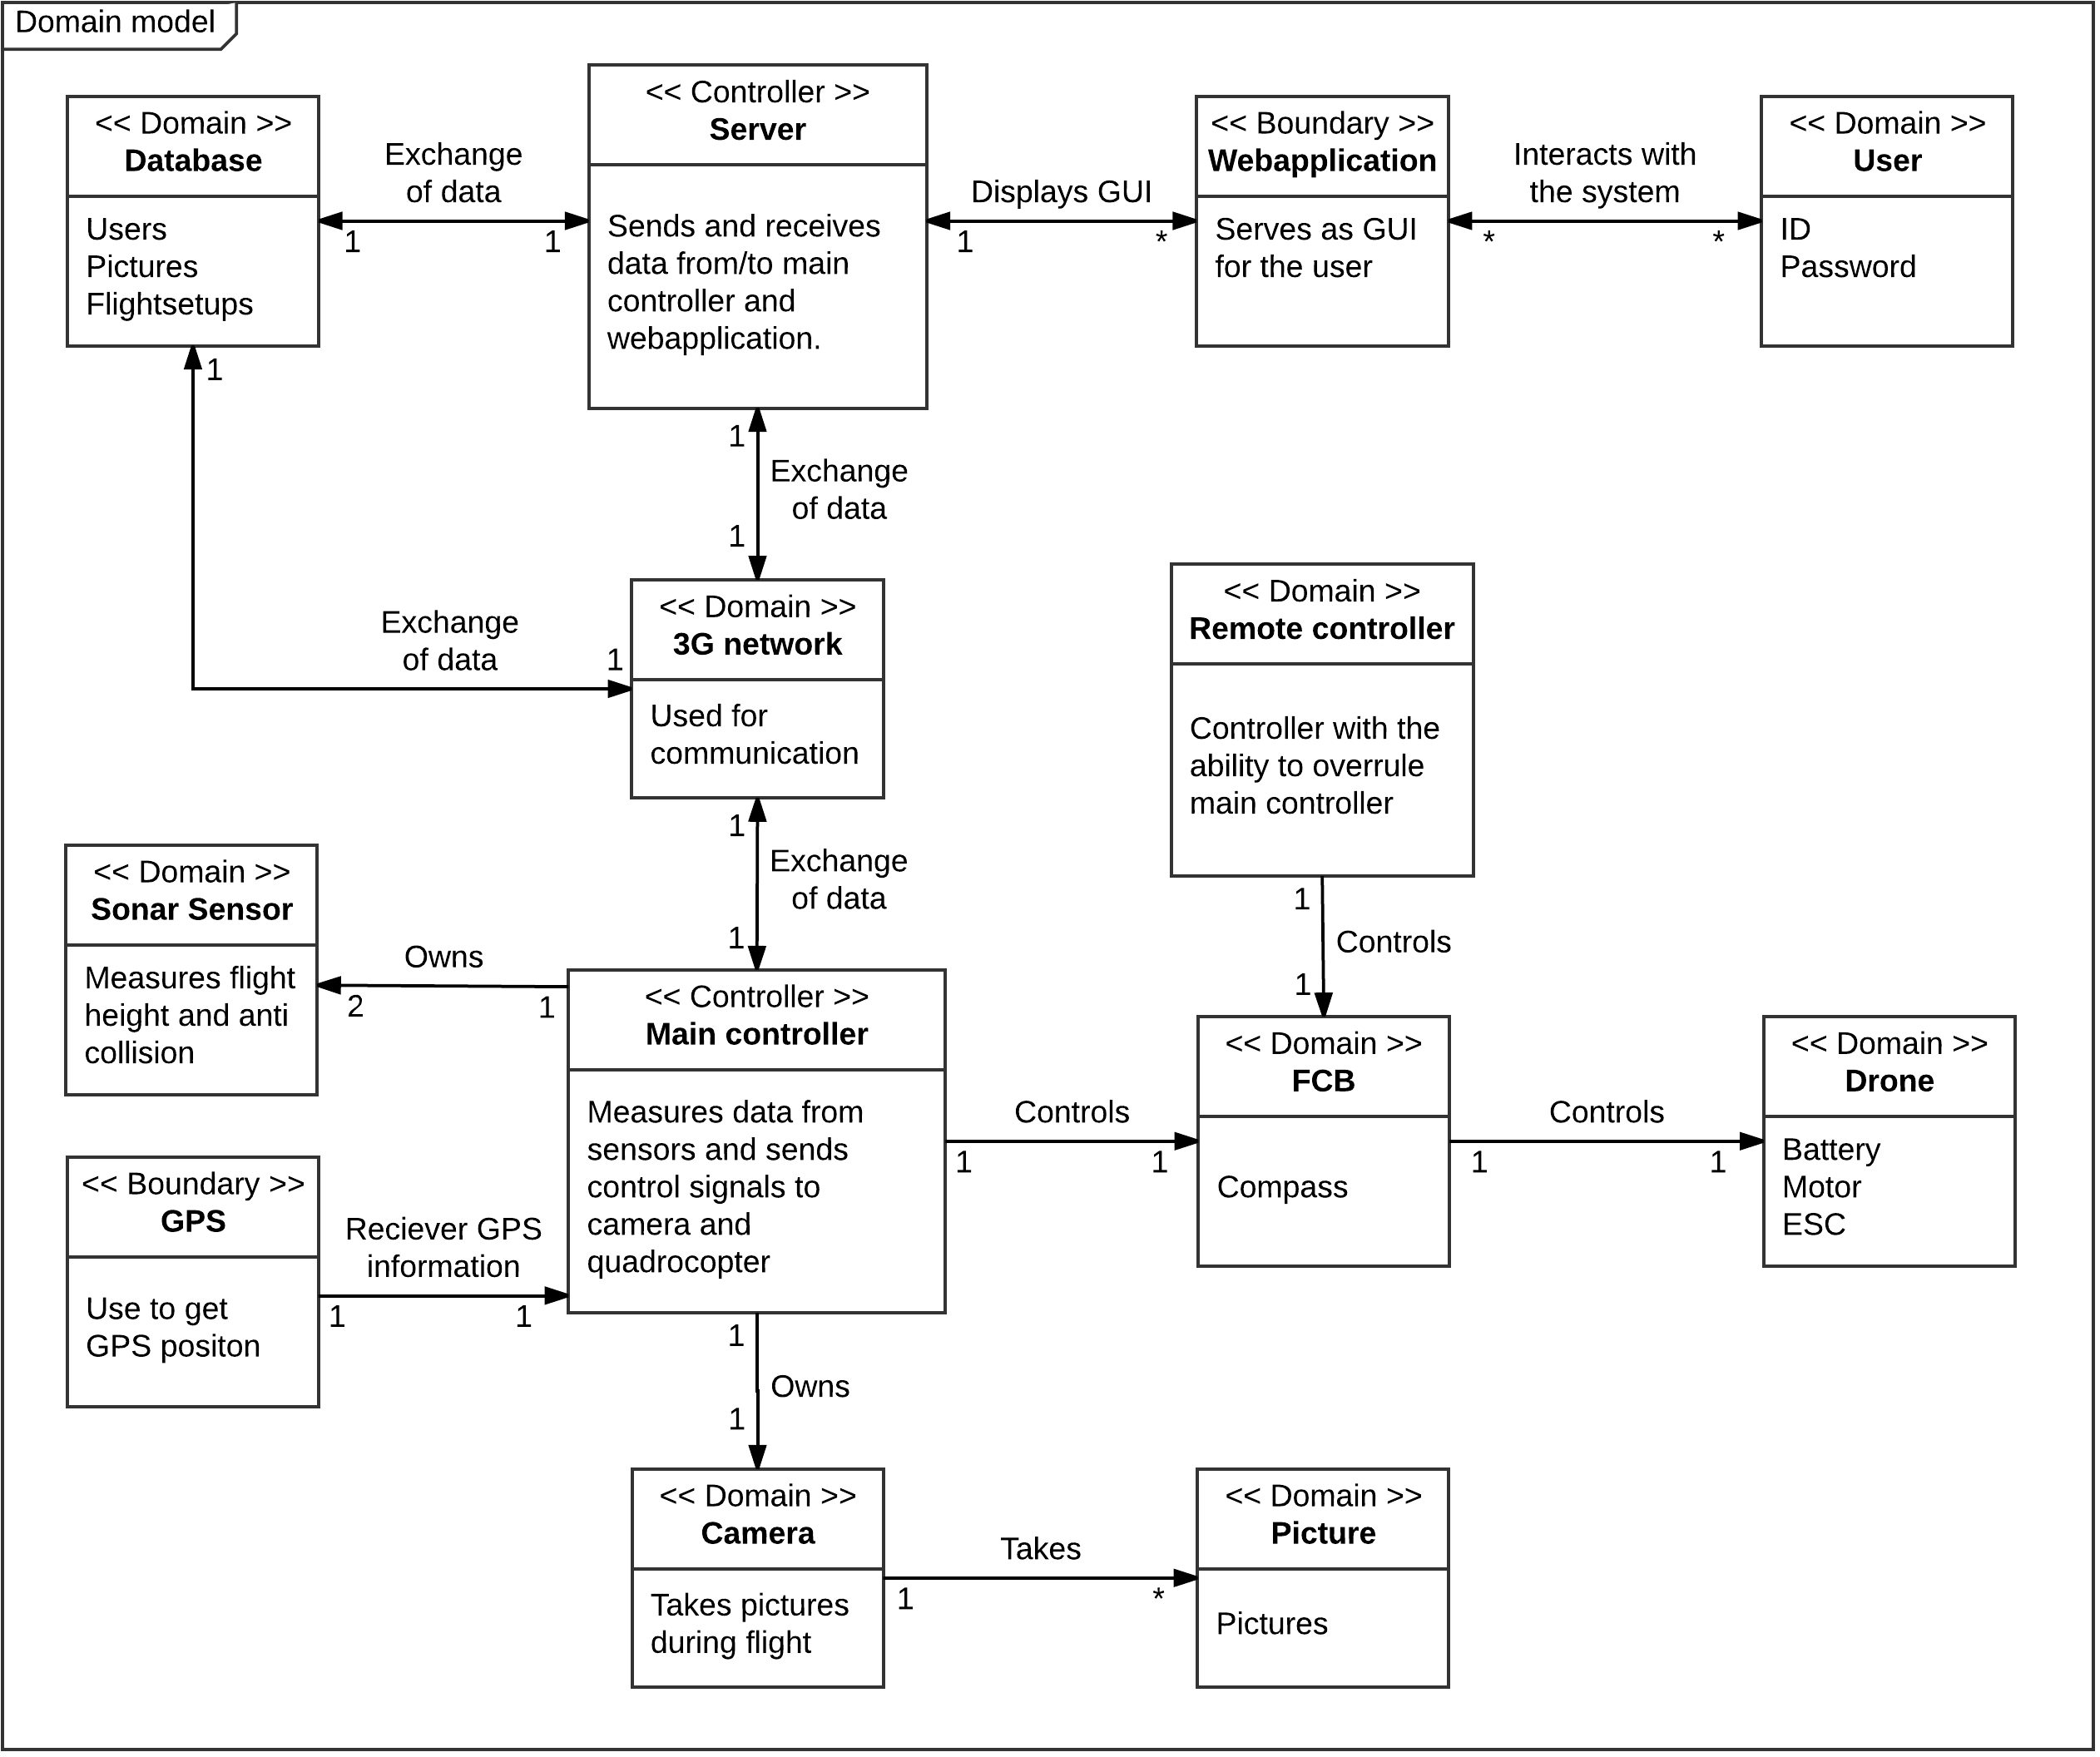
\includegraphics[width=1\textwidth]{Billeder/domain_model.png}
	\caption{Domain model}
	\label{fig:domain}
\end{figure}


\newpage

Efter at have udarbejdet kravspecifikation, systemskitse og domain model, var der formet en ide om hvordan systemet skulle fungere. I det følgende beskrives hvordan systemarkitekturen er udformet. 


Systemarkitekturen er udført ved brug af SysML og UML diagrammer. 
SysML bruges til beskrivelse af systemets hardware i blokke og som samlet system. Ud fra N + 1 og applikations modellen udformes UML diagrammer, der bruges til beskrivelse af systemets software. 
Foruden SysML og UML diagrammer benyttes en række andre diagrammer, i det følgende beskrives nogle af de mest centrale diagrammer.\\


\textbf{Use case}\\
Use cases og tilhørende diagrammer er benyttet i projektforløbets indledende faser. De bruges til at definere systemets kunnen og opdele systemet i mindre dele. Use cases har i høj grad fungeret som et omdrejningspunkt, hvorfra alt funktionalitet udspringer. \\


\textbf{SysML}\\
Der er benyttet to slags SysML diagrammer til dokumentation af systemets hardware. Block definition diagrammer (bdd'er) er brugt til at identificere og beskrive systemets hardware blokke og deres indbyrdes forhold. Internal block diagrammer (ibd'er) er brugt til at vise de identificerede blokkes interne og eksterne forbindelse, hvordan blokkene kommunikerer og hvilke signaler der flyder imellem dem. \\


\textbf{UML}\\
Der er benyttet fire slags UML diagrammer til dokumentation af systemets software.
På baggrund af use cases og domain modellen udformes pakkediagrammer, der bruges til at beskrive ansvarsområder i systemet. Sekvensdiagrammer bruges til at identificere systemets klasser, klassernes metoder samt timing i systemet. Klasser samt tilhørende metoder og attributter beskrives ved hjælp af klassediagrammer. State machines bruges til at beskrive flow mellem forskellige states. 


\newpage

\subsection{Hardware}
I dette afsnit beskrives hvordan systemets hardwarearkitektur er udformet vha. SysML diagrammer. Indledningsvis bruges block definition diagrammer til at identificere og beskrive systemets blokke. Senere åbnes udvalgte blokke og de interne og eksterne forbindelser vises med internal block diagrammer. 


\subsubsection*{Block definition diagram}

Det overordnede bdd på figur \ref{fig:bdd_asd} viser hvilke hardware blokke systemet består af, samt hvilke parts blokkene indeholder.

\begin{figure}[H]
	\centering
	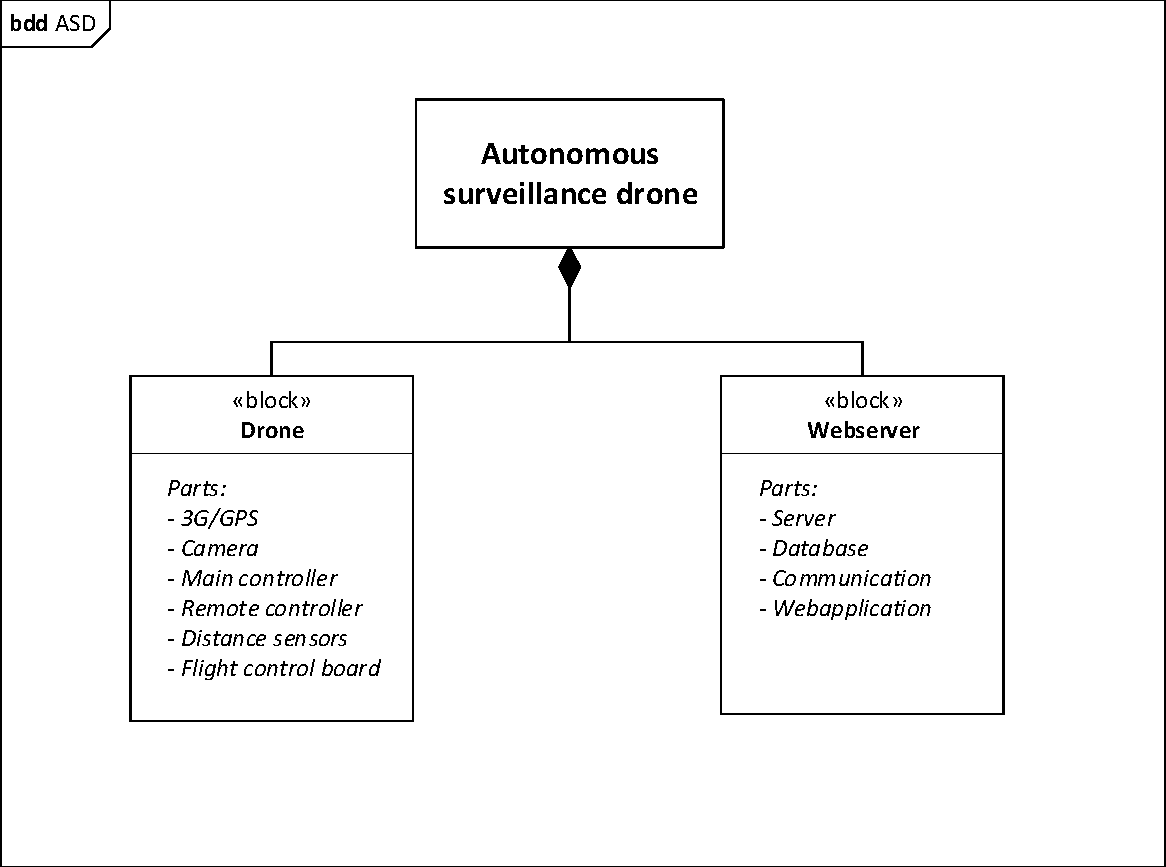
\includegraphics[width=1.0\textwidth]{Billeder/Projektbeskrivelse/bdd_overordnet.pdf}
	\caption{Overordnet bdd for systemet}
	\label{fig:bdd_asd}
\end{figure}

\textbf{Drone} \\
Drone blokken indeholder alle de hardwareenheder der giver funktionalitet til drone. Beskrivelse af de eksterne og interne forbindelser mellem de forskellige parts er beskrevet nærmere med ibd'er. \\

\textbf{Webserver} \\
Webserver blokken indeholder server, database, communication og webapplikationen.

\newpage

\subsubsection*{Internal block diagram}
\vspace{-0.3cm}	

På figur \ref{fig:ibd_asd} vises et overordnet ibd for systemet. Det overornede ibd viser hvordan systemets største blokke kommunikerer med hinanden og hvilken type signaler der anvendes mellem blokkene. 

\begin{figure}[H]
	\centering
	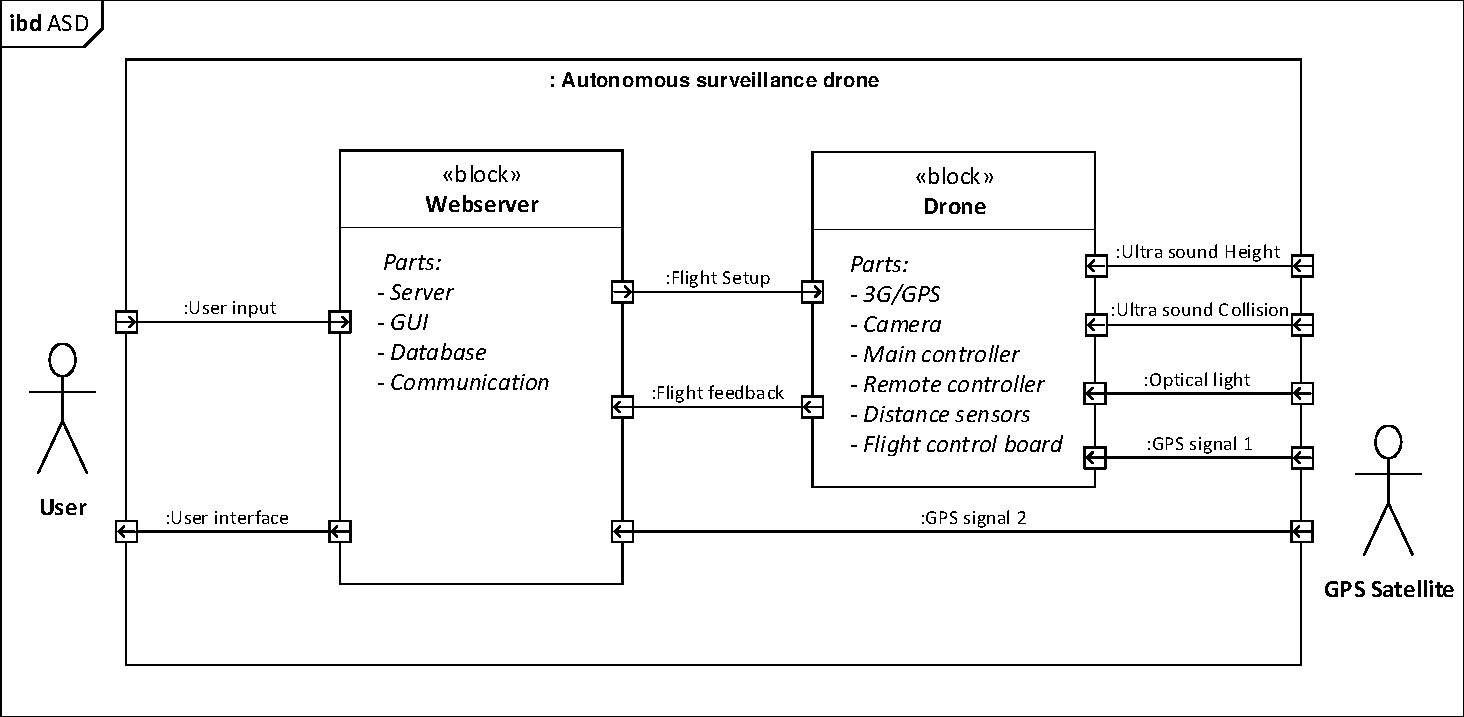
\includegraphics[width=1\textwidth]{Billeder/Projektbeskrivelse/ibd1_overordnet.pdf}
	\caption{Overordnet ibd for systemet}
	\label{fig:ibd_asd}
\end{figure}

Da drone blokken er stor og indeholder mange part kræves yderlige beskrivelse. På den følgende side åbnes drone blokken og de interne forbindelser i blokken vises.

\newpage


På figur \ref{fig:ibd_drone} vises et ibd, der går mere i dybden med drone blokken. ibd'et åbner drone blokken og viser hvordan parts i drone blokken kommunikerer med hinanden. 

\begin{figure}[H]
	\centering
	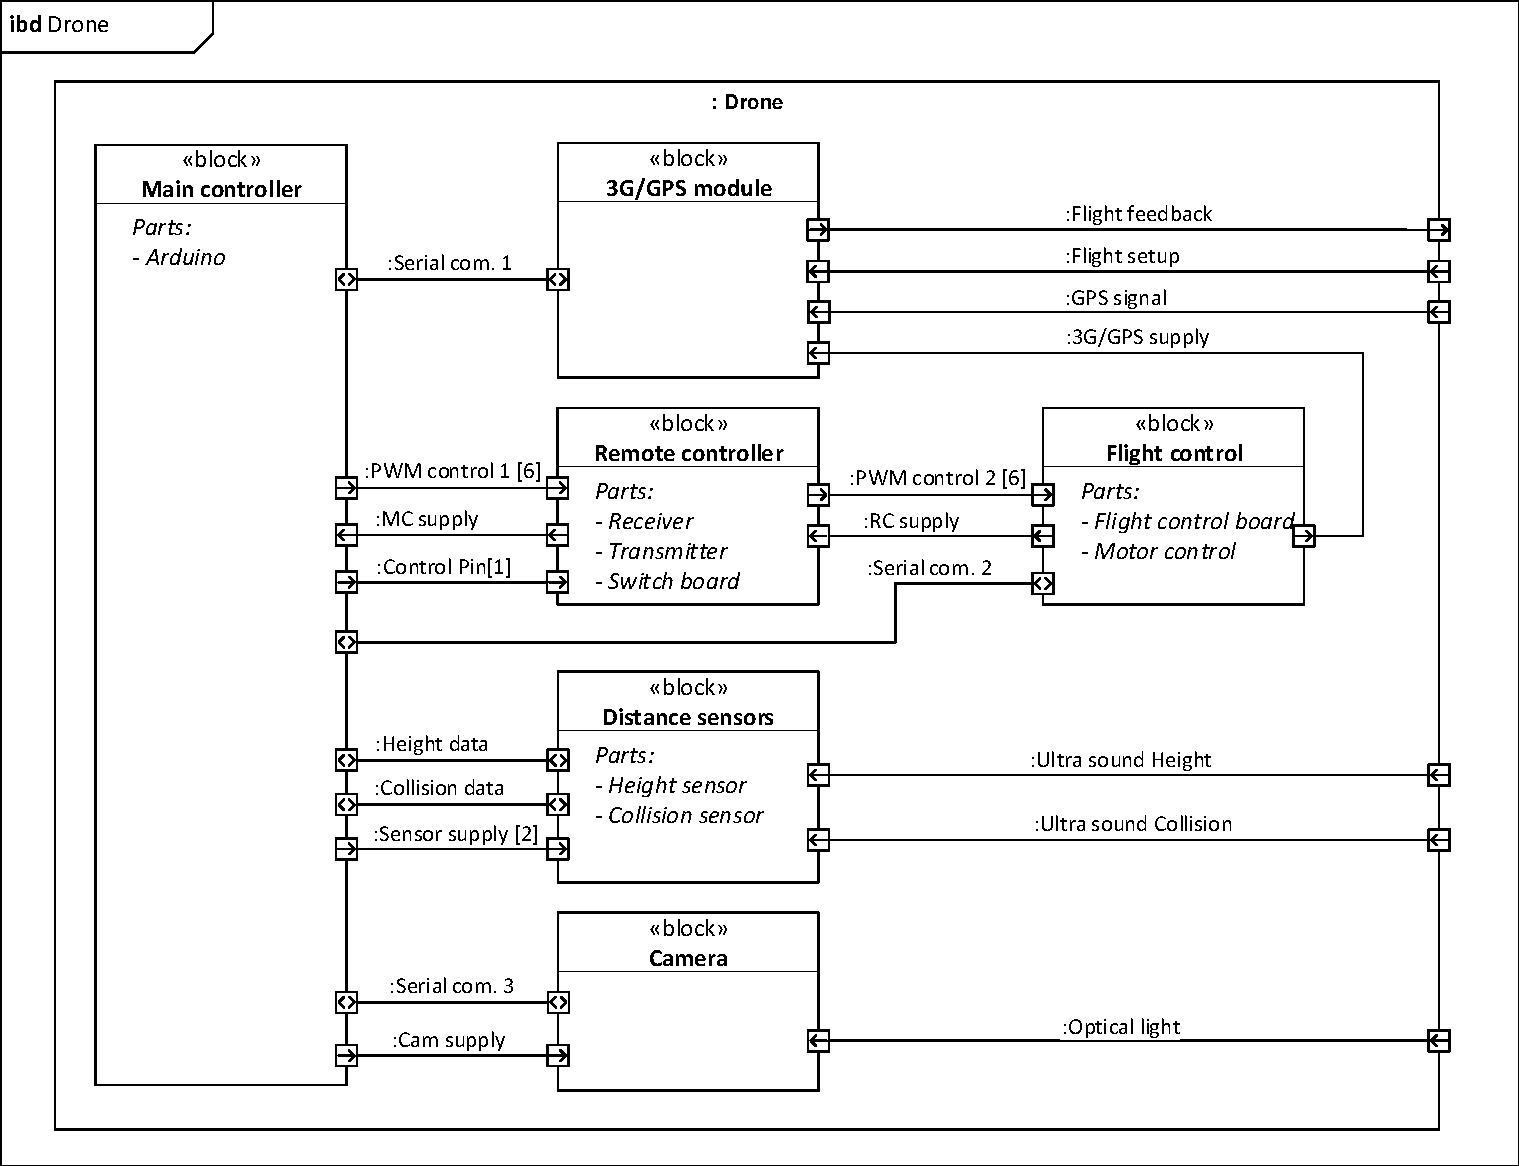
\includegraphics[width=1\textwidth]{Billeder/Projektbeskrivelse/ibd2_drone.pdf}
	\caption{ibd drone}
	\label{fig:ibd_drone}
\end{figure}


For yderlige beskrivelser af parts fra drone blokken henvises til ibd'er i hardwarearkitektur [3].
Der vises ikke udvidede ibd'er for webserver, da webserver ikke indeholder hardware og derfor beskrives nærmere ved brug af UML diagrammer i software afsnittet.



\newpage

\subsection{Software}

I dette afsnit beskrives hvordan softwarearkitekturen ved brug af N+1 og applikations modellen tager udgangspunkt i use cases og ender ud i detaljerede klassedigrammer. 
   
\subsubsection*{Pakkediagrammer}
\vspace{-0.3cm}	
Indledningsvis identificeres pakkediagrammer ud fra use cases og domain modellen. På figur \ref{fig:package_drone} vises et pakkediagram tilhørende dronens software. Pakkerne i pakkediagrammet bruges til at definere de forskellige ansvarsområder i systemts software. For nærmere beskrivelser af pakkediagrammer over systemets software henvises til logical view [4].
 
\begin{figure}[H]
	\centering
	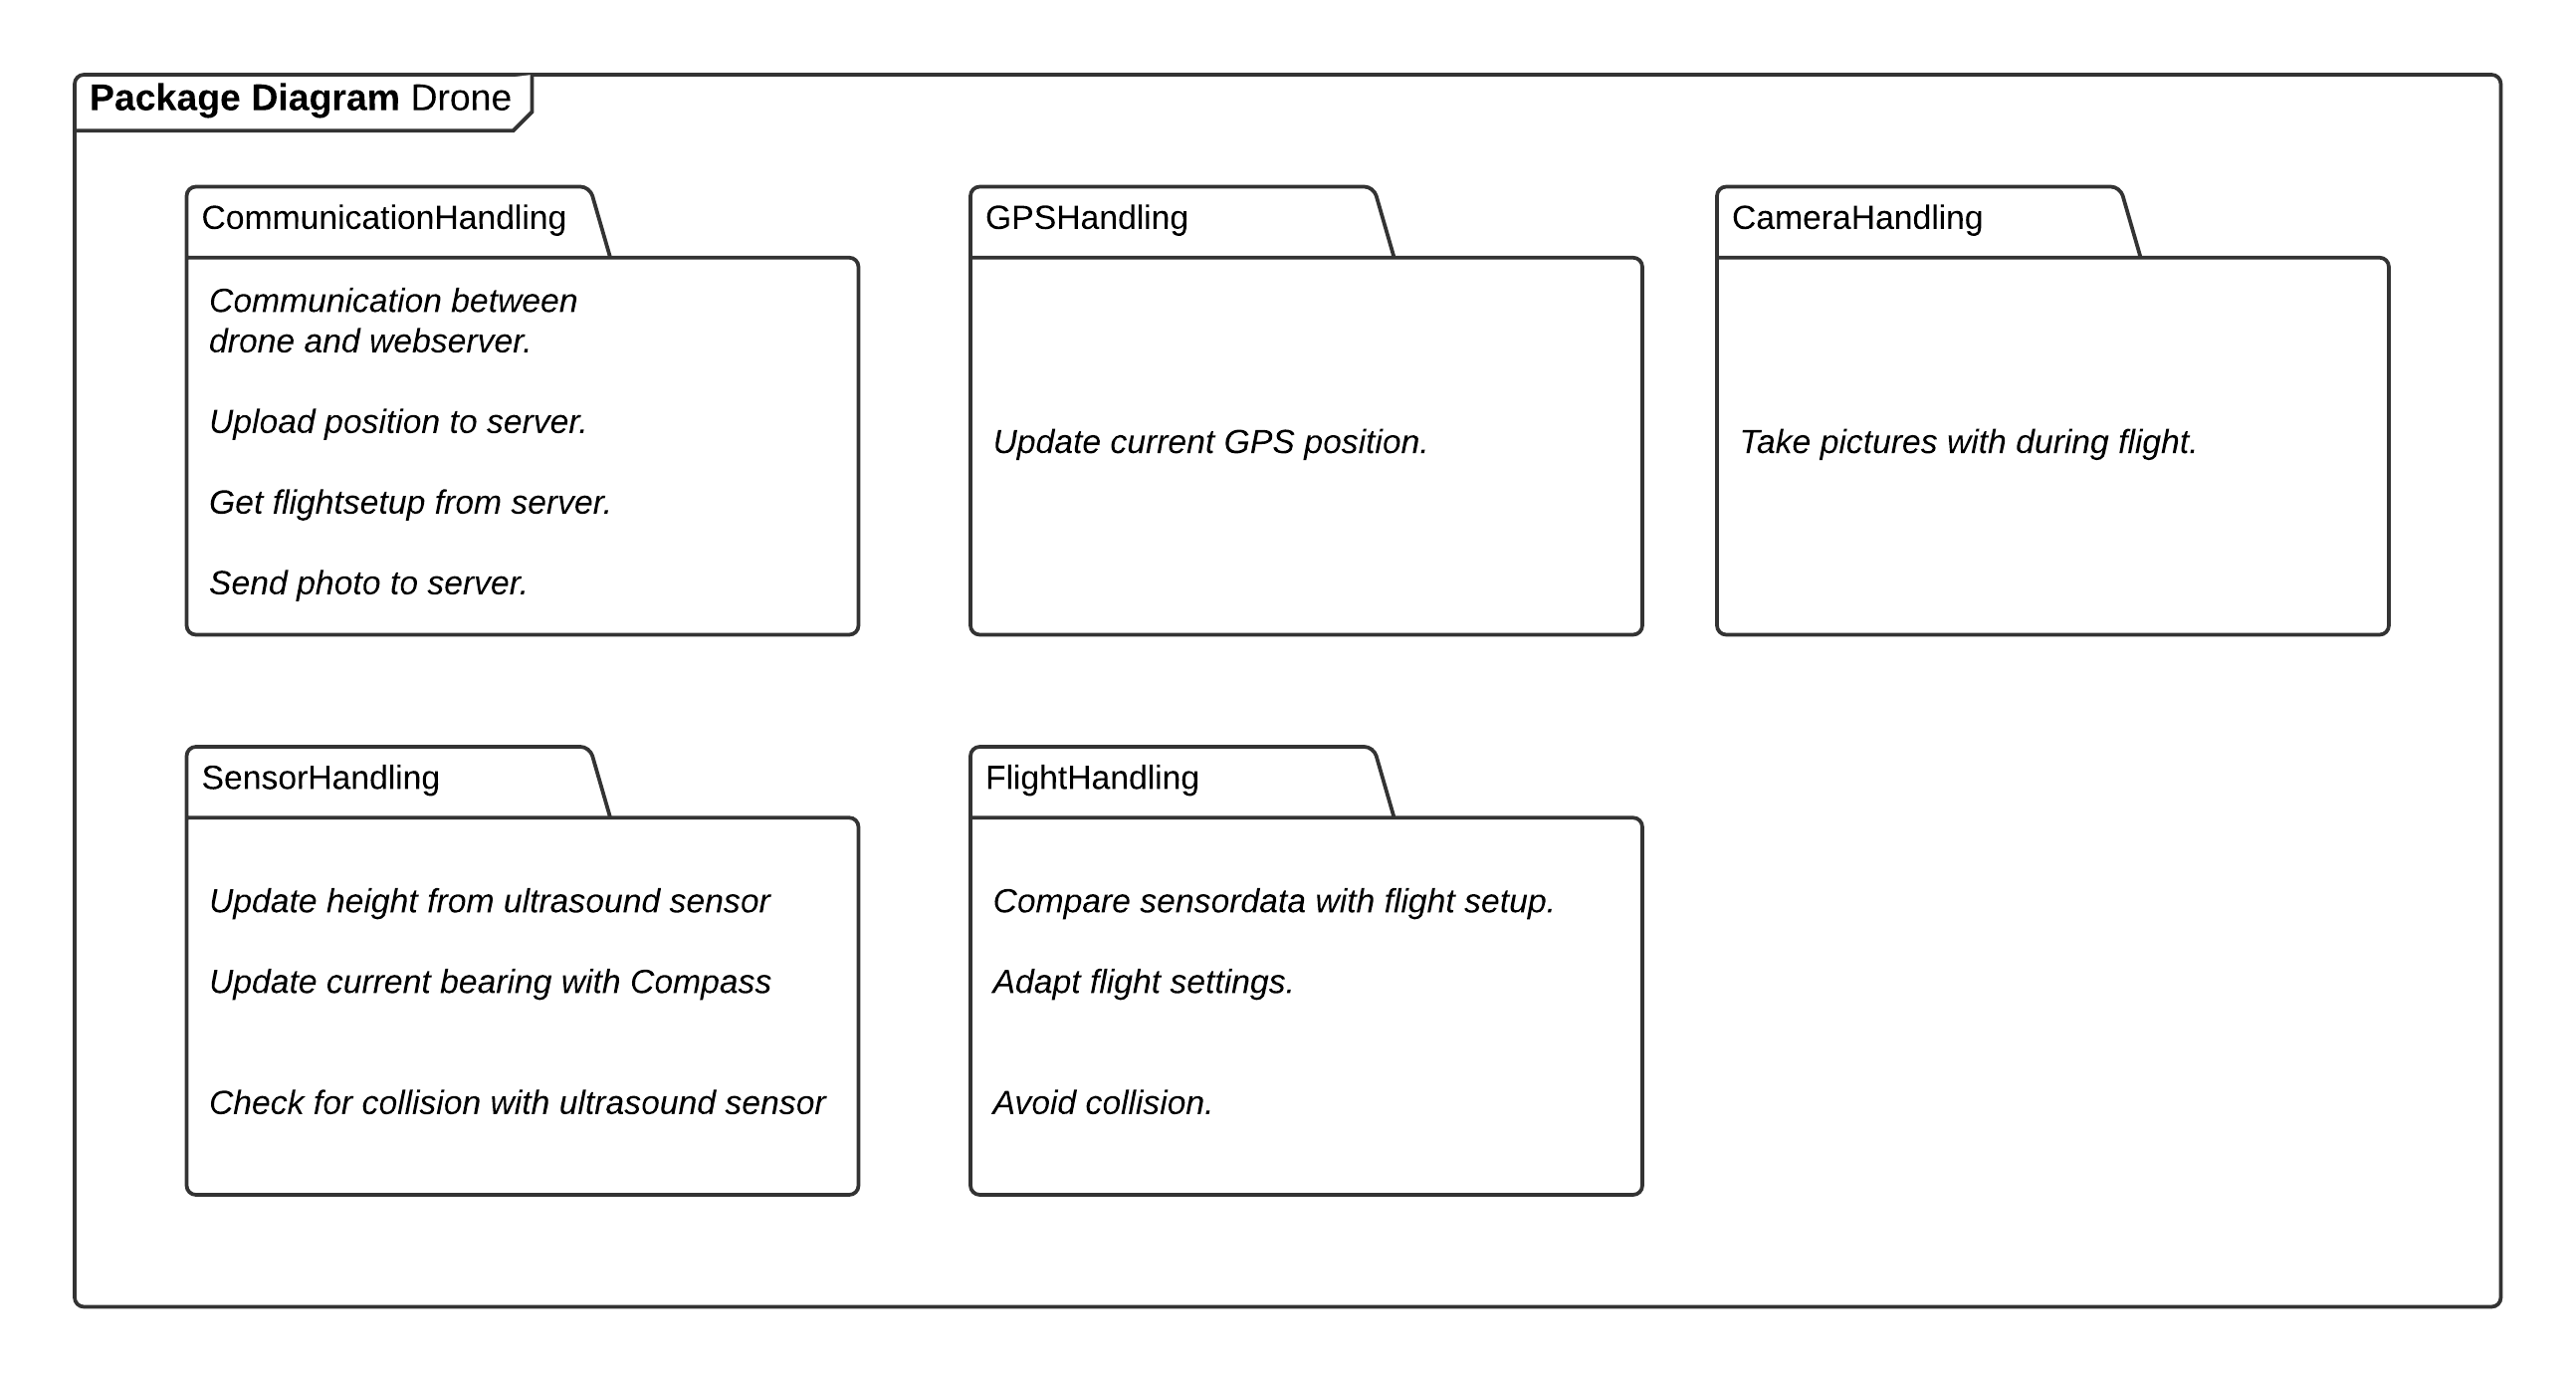
\includegraphics[width=1\textwidth]{Billeder/Projektbeskrivelse/Packagediagram_drone}
	\vspace{-0.9cm}	
	\caption{Overordnet pakkediagram for drone}
	\label{fig:package_drone}
\end{figure}

\newpage

\subsubsection*{Sekvensdiagrammer}
\vspace{-0.3cm}	

Efter at have udformet pakkediagrammer påbegyndes udformning af sekvensdiagrammer. Disse diagrammer bruges til at identificere softwareklasser, klassernes metoder, klassernes indbyrdes forhold, samt timing i systemet. Enheder der indgår i sekvensdiagrammerne tages ud fra domain modellen. 

Sekvensdiagrammet på figur \ref{fig:login_flysetting} viser et eksempel på en use case omsat til et sekvensdiagram. Sekvensdiagrammet bruges til overordnet at vise hvordan bruger interagerer med webapplikation når der laves ny flyveopsætning. For yderlige beskrivelser af sekvensdiagrammer tilhørende systemet henvises til logical view [4].

 
\begin{figure}[H]
	\centering
	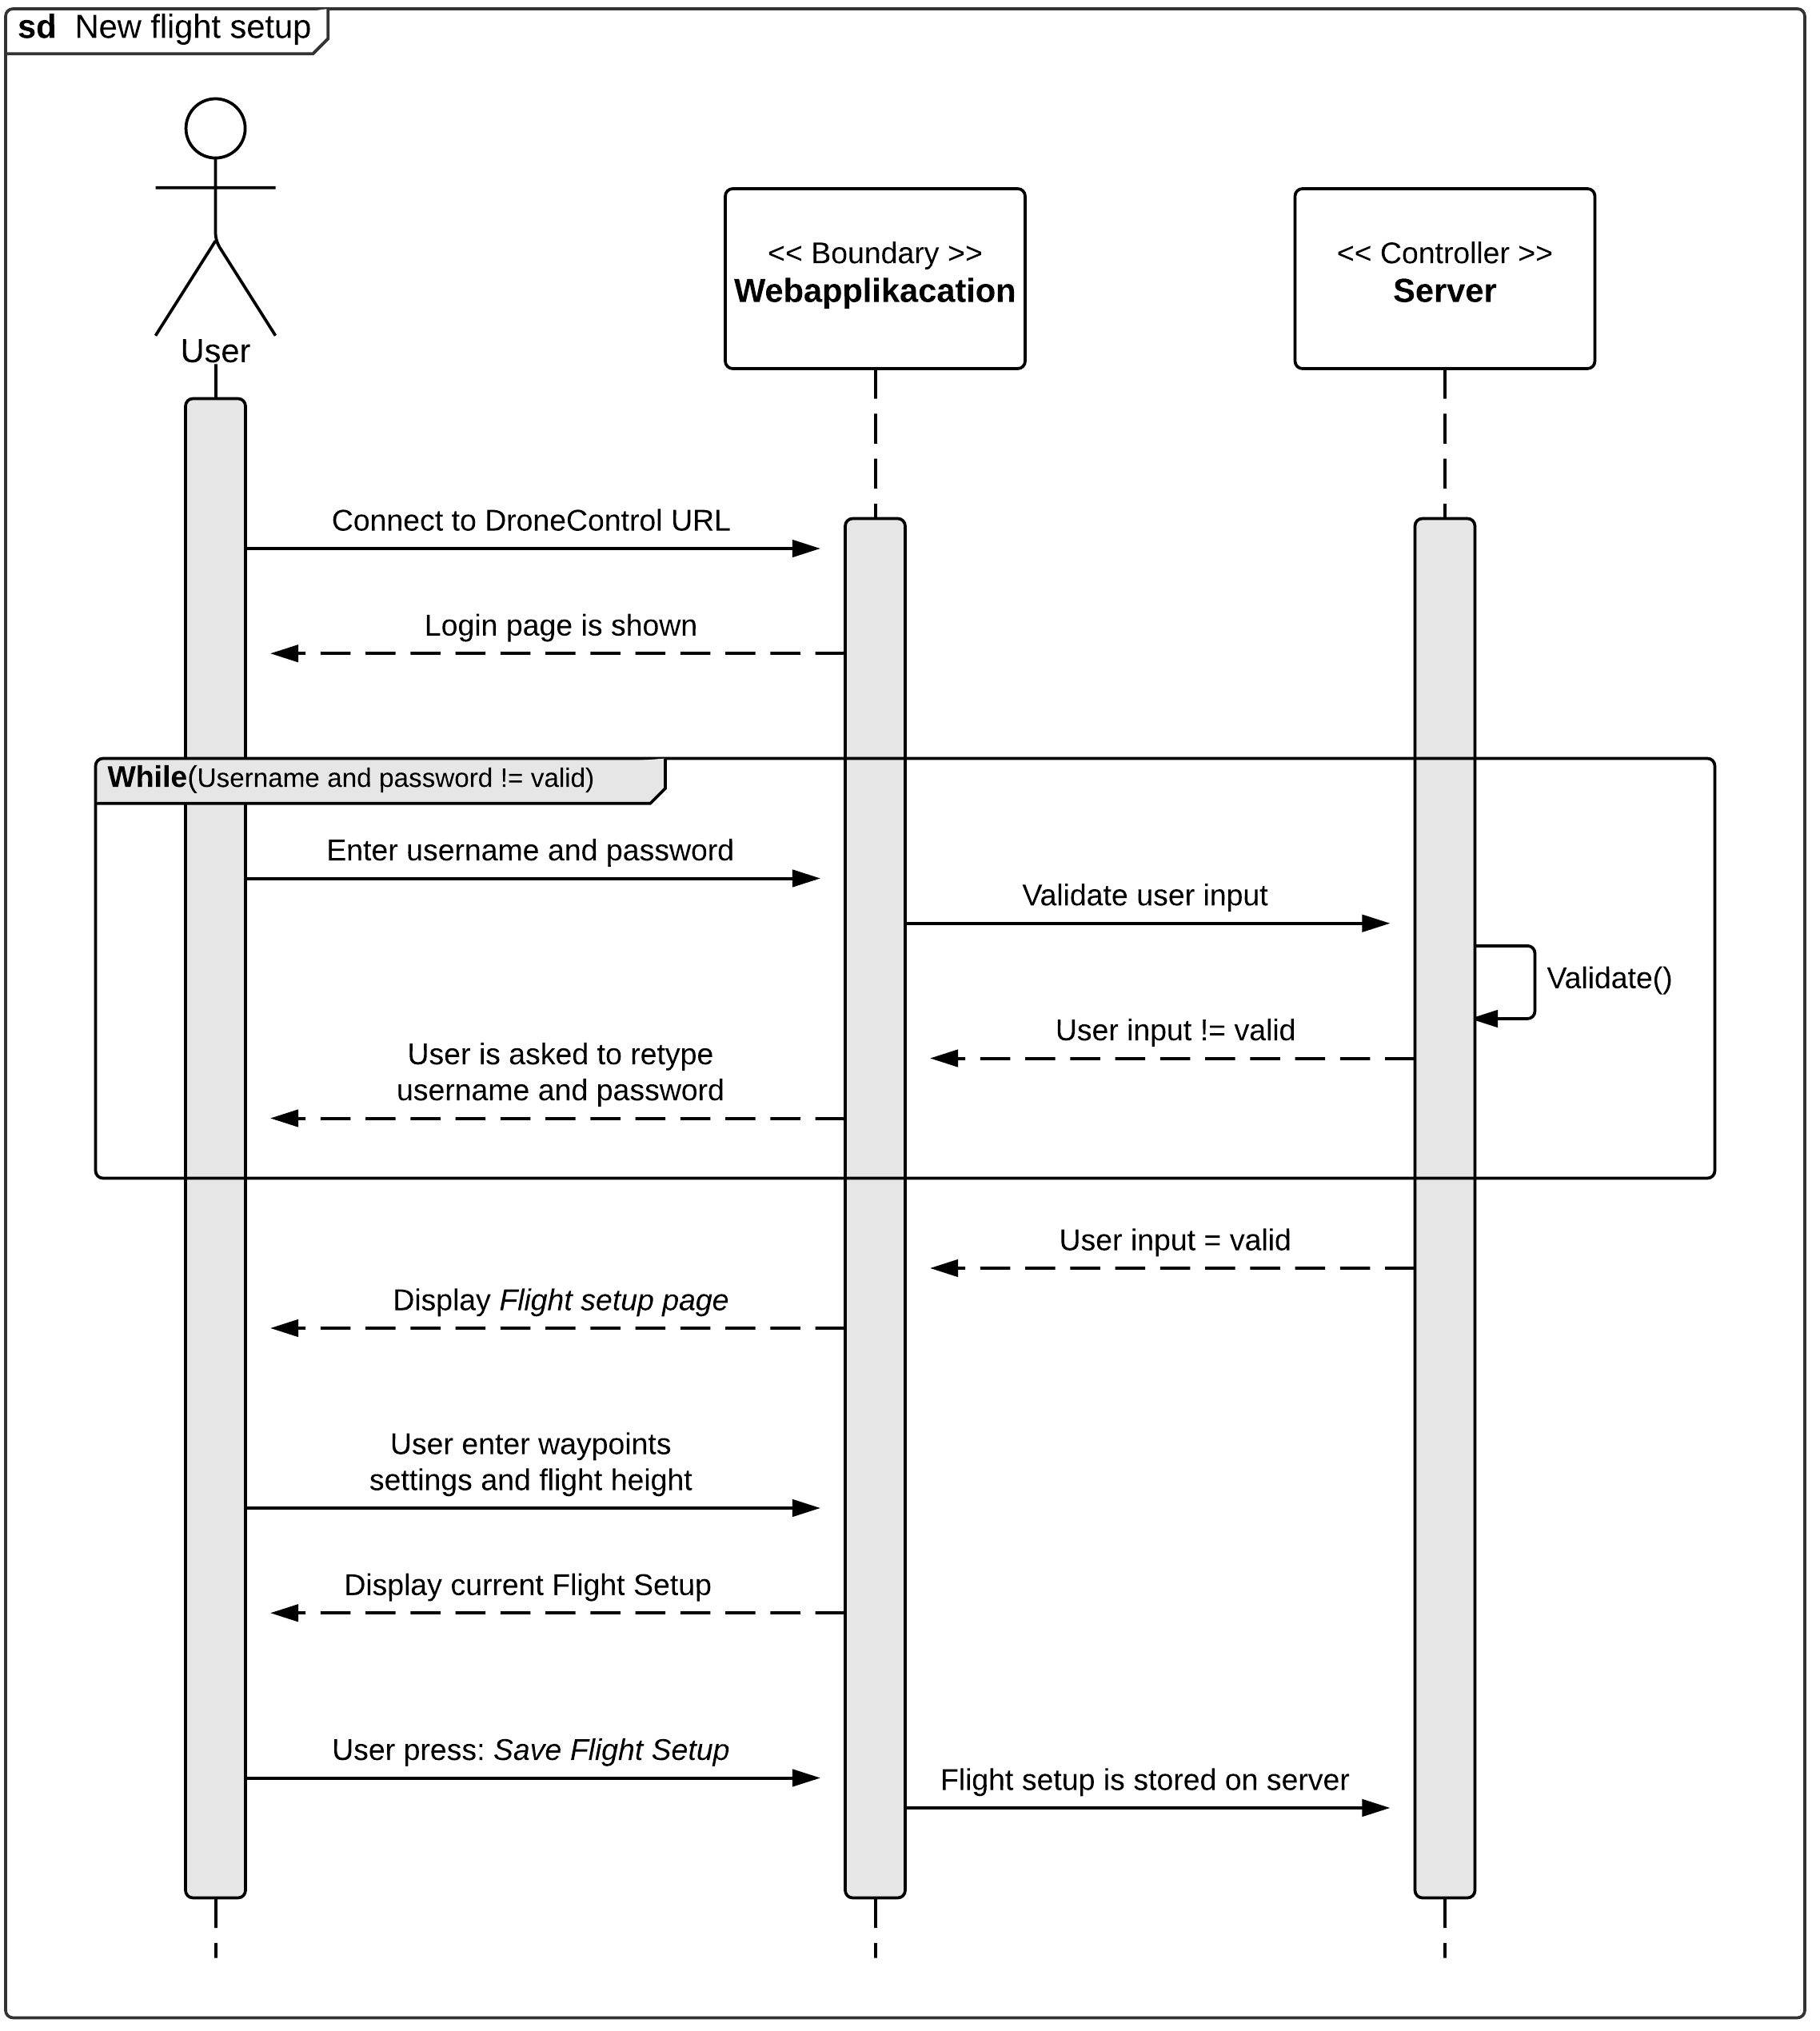
\includegraphics[width=1\textwidth]{Billeder/sekvens.png}
	\vspace{-0.6cm}	
	\caption{Sekvensdiagram - ny flyveopsætning}
	\label{fig:login_flysetting}
\end{figure}

\newpage
\subsubsection*{Klassediagrammer}
\vspace{-0.3cm}	

Efter at have udformet sekvensdiagrammer er der opbygget et vist kendskab til de forskellige klasser, deres metoder og deres indbyrdes forhold. For på overskuelig vis at illustrere og beskrive systemets softwareklasser laves klassediagrammer.

På figur \ref{fig:class_drone} vises et klassediagram tilhørende dronens software. Bemærk at klassediagrammet er fra første iteration, hvilket betyder det er relativt lille og ikke indeholder så mange klasser og metoder. For mere information om de enkelte klasser og deres ansvarsområder henvises til logical view [4].

\begin{figure}[H]
	\centering
	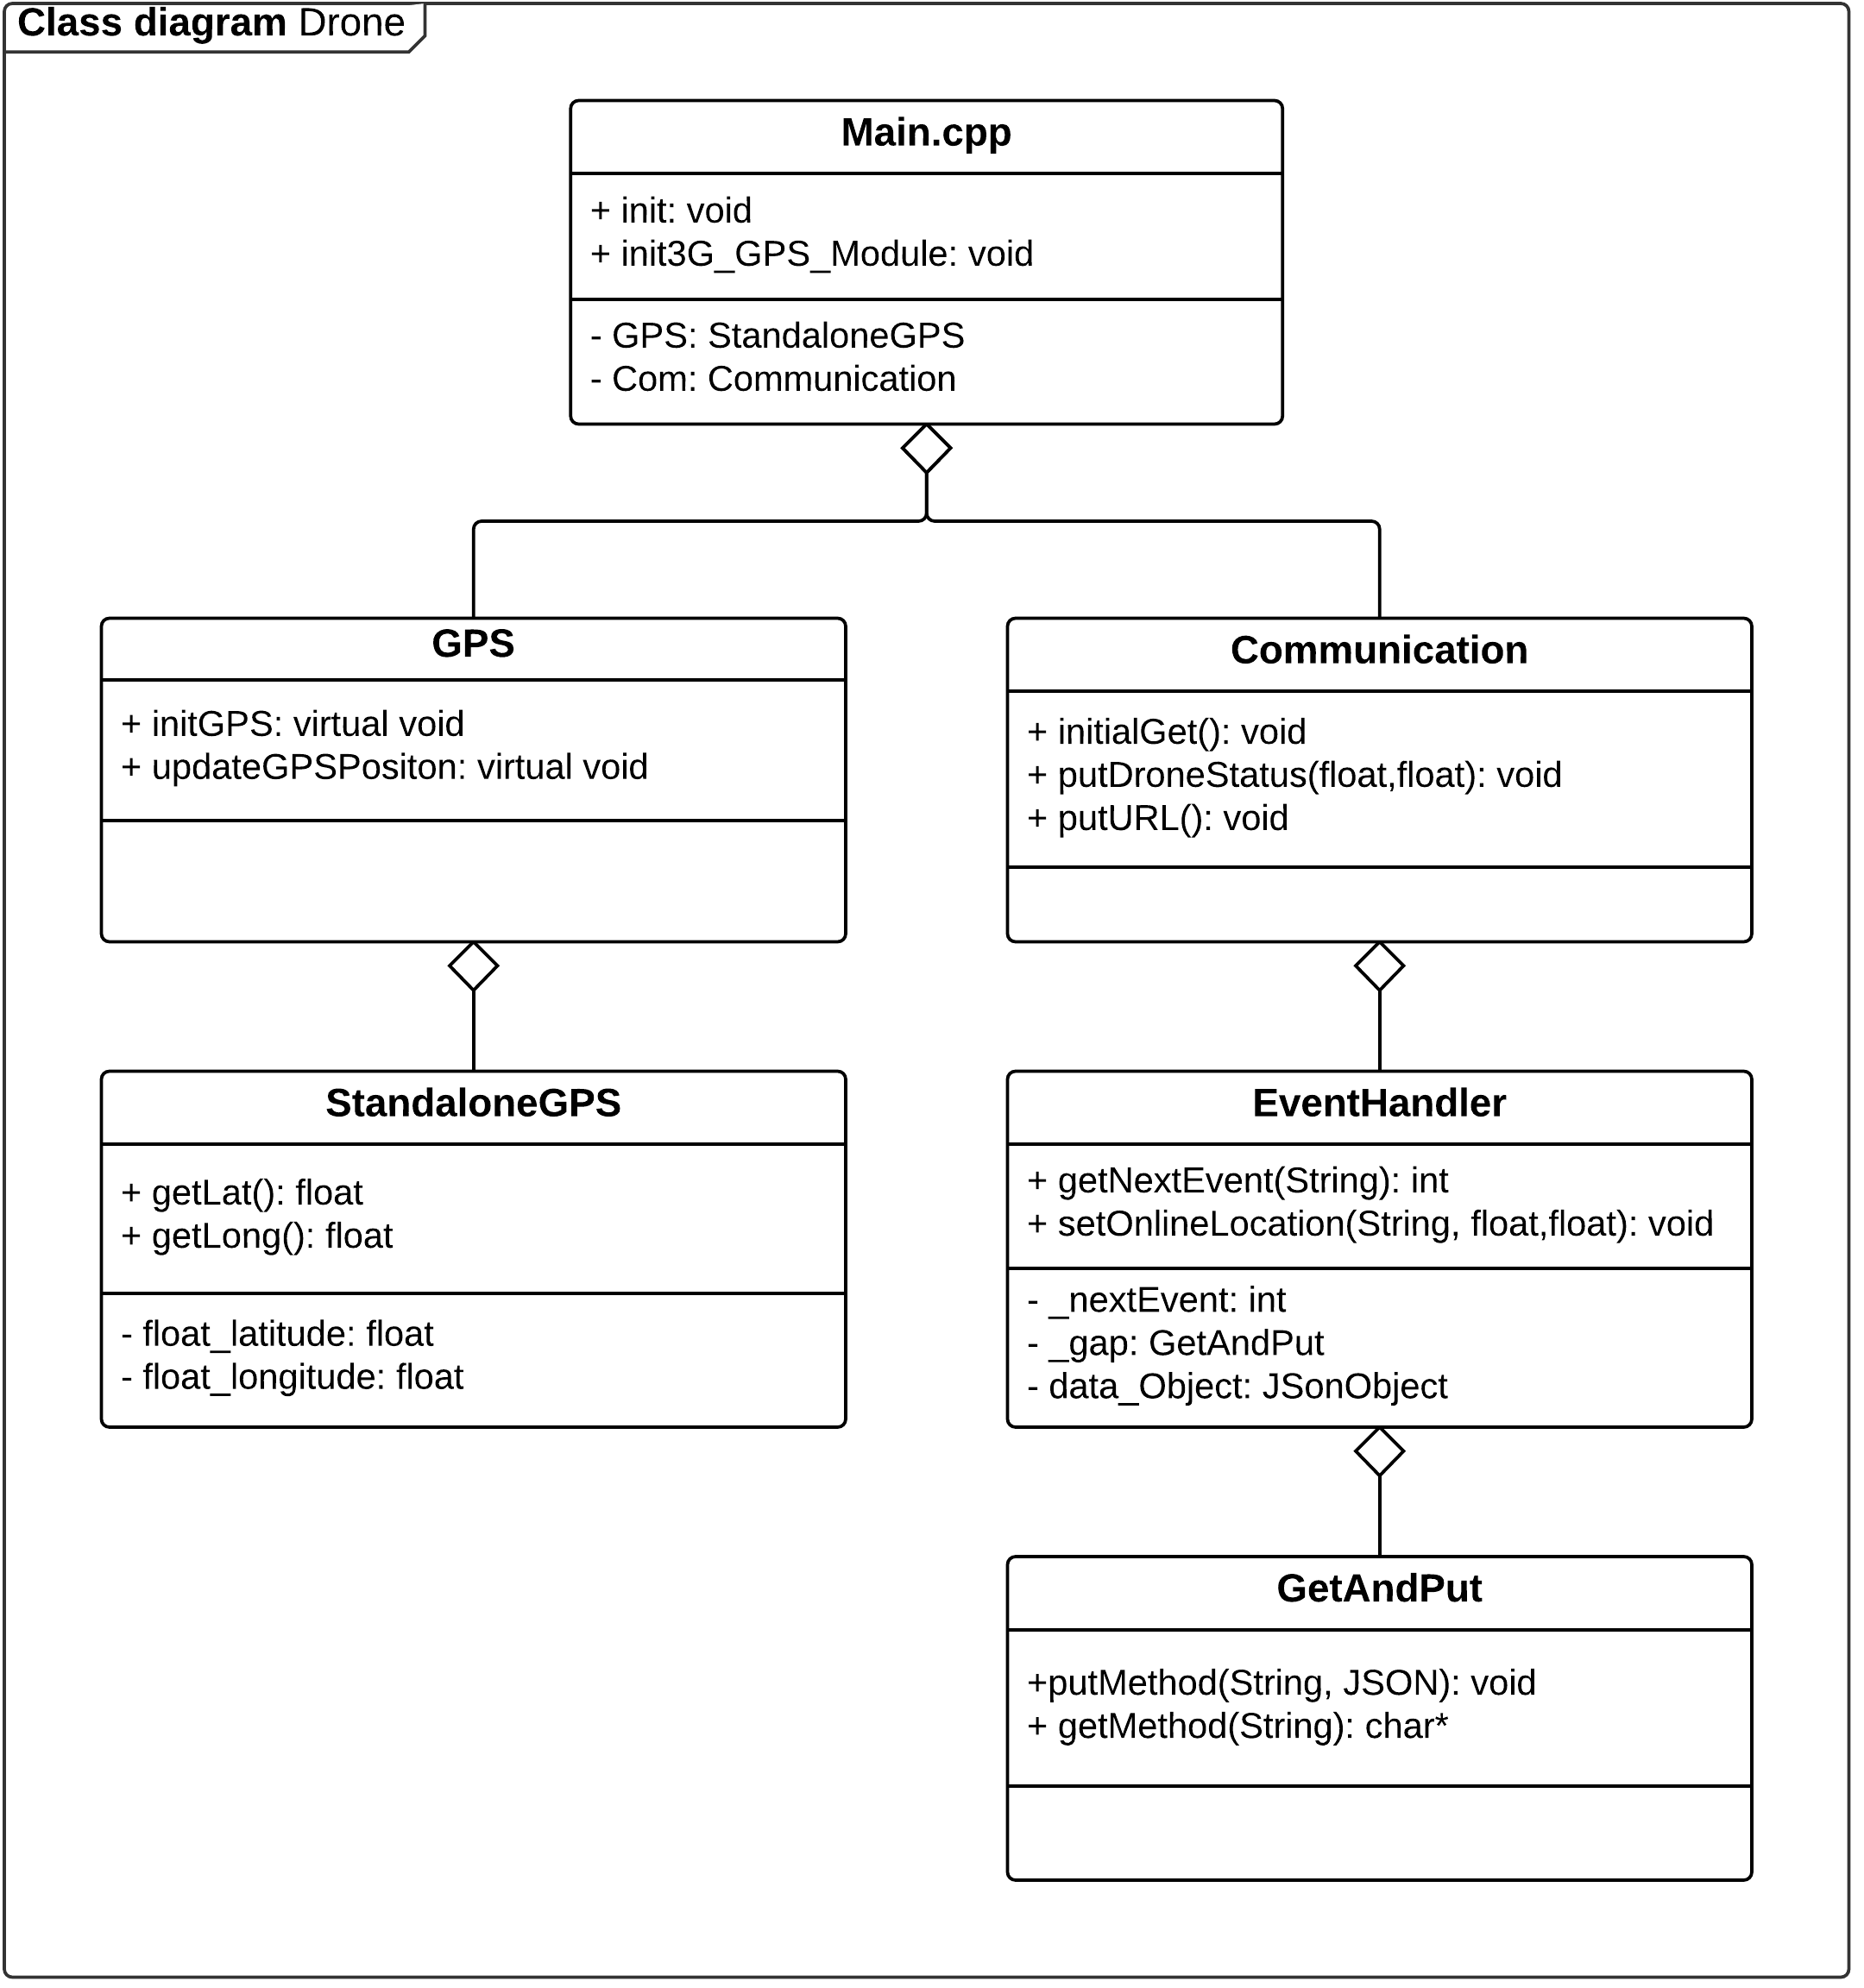
\includegraphics[width=1\textwidth]{Billeder/classdiagram.png}
	\vspace{-0.6cm}	
	\caption{Klassediagram drone}
	\label{fig:class_drone}

\end{figure}


%%%%%% Design %%%%%%
\section{Design}

I dette afsnit beskrives systemets design. Systemet indeholder overordnet set de tre enheder drone, server og webapplikation samt en kommunikations protokol derimellem. Drone bruges til at overvåge og tage billeder, server står for håndtering af data, og webapplikation er systemets grænseflade til bruger. Mellem drone/server og webapplikation/server gøres brug af HTTP protokollen til kommunikation og udveksling af data.



\subsection{Drone}

Systemets bruger er ansvarlig for at lave flyveopsætninger, som indeholder informationer om det område drone skal overvåge.

Når drone tændes skal den løbende og uden menneskelig indblanding kontrollere om der er en ny flyveopsætning tilgængelig på server. Hvis der er en ny flyveopsætning tilgængelig hentes den, og en ny flyvning påbegyndes. 

Under flyvning flyver drone på egen hånd til de definerede GPS positioner. Afhængig af om bruger har valgt om der skal tages billeder eller ej, tager dronen billeder som via mobilt netværk sendes til server. 
Under flyvning kontrollerer drone løbende egen GPS position, flyvehøjde og flyveretning. Dette gør dronen for løbende at kunne tilpasse flyvehøjde og orientering og for at kunne sende information om nuværende GPS position til server.

På figur \ref{fig:class_drone} vises et simplificeret klasse diagram for drone. I det viste klassediagram vises softwareklasser og deres indbyrdes forhold. For yderlige information om de enkelte klasser, deres metoder og deres ansvarsområder henvises til logical view i \textit{Systemarkitektur og Design} i dokumentationen. [xx]

\begin{figure}[H]
\centering
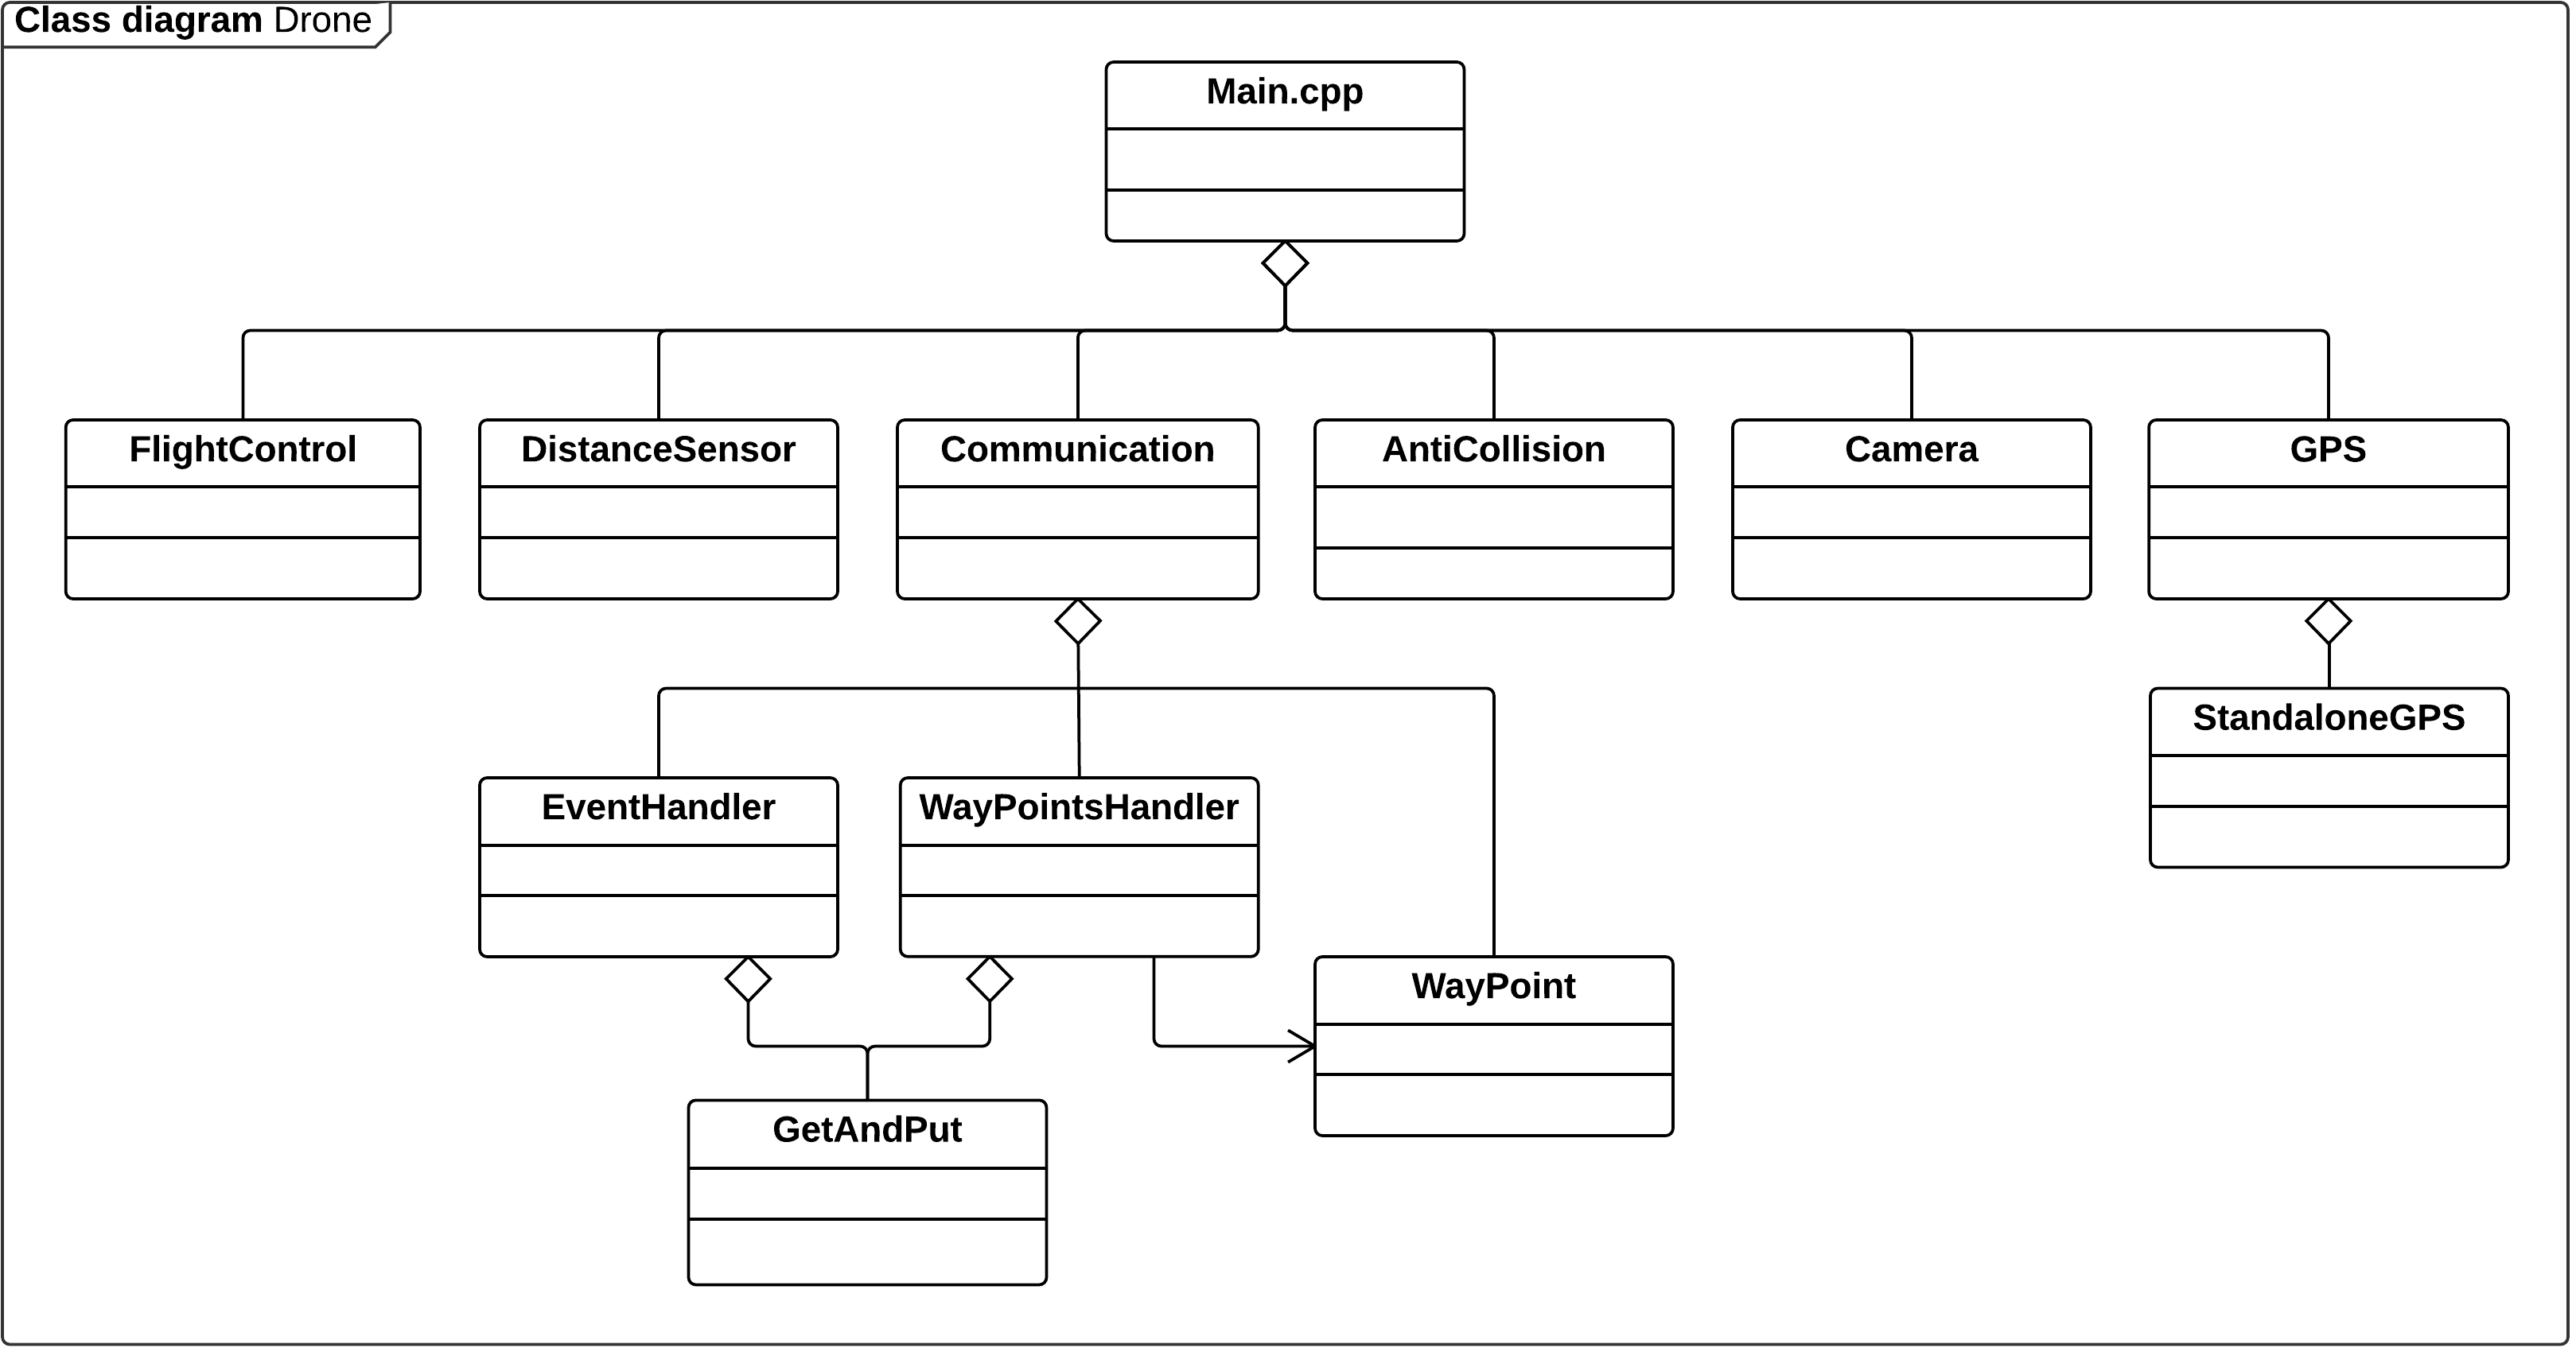
\includegraphics[width=1\textwidth]{Billeder/Design_Class_drone.png}
\vspace{-0.5cm}
\caption{Klassediagram drone}
\label{fig:class_drone}
\end{figure}


\newpage 

\subsection{Server}

Server består af SQLite database med et tilhørende REST API. I SQLite databasen gemmes og hentes løbende information om systemets brugere, samt information om flyveopsætninger, flyveruter og billeder.  

Server er en passiv enhed, som er ansvarlig for håndtering af systemets data. Server tager aldrig initiativ til udveksling af data, den står i stedet og venter på at blive igangsat af enten drone eller webapplikation.

For systemets bruger kan det se ud som om udveksling af data og information går direkte fra webapplikation til drone eller omvendt. Men reelt set er webapplikation og drone aldrig i direkte kontakt med hinanden. I stedet går al kommunikation til og fra server via HTTP protokollen. 

På figur \ref{fig:deployment_diagram} ses et deployment diagram, der viser hvordan drone og webapplikation kommunikerer med server for at hente og gemme information. For yderlige information om server og tilhørende SQLite database henvises til data view i \textit{Systemarkitektur og Design} i dokumentationen [xx].

\begin{figure}[H]
\centering
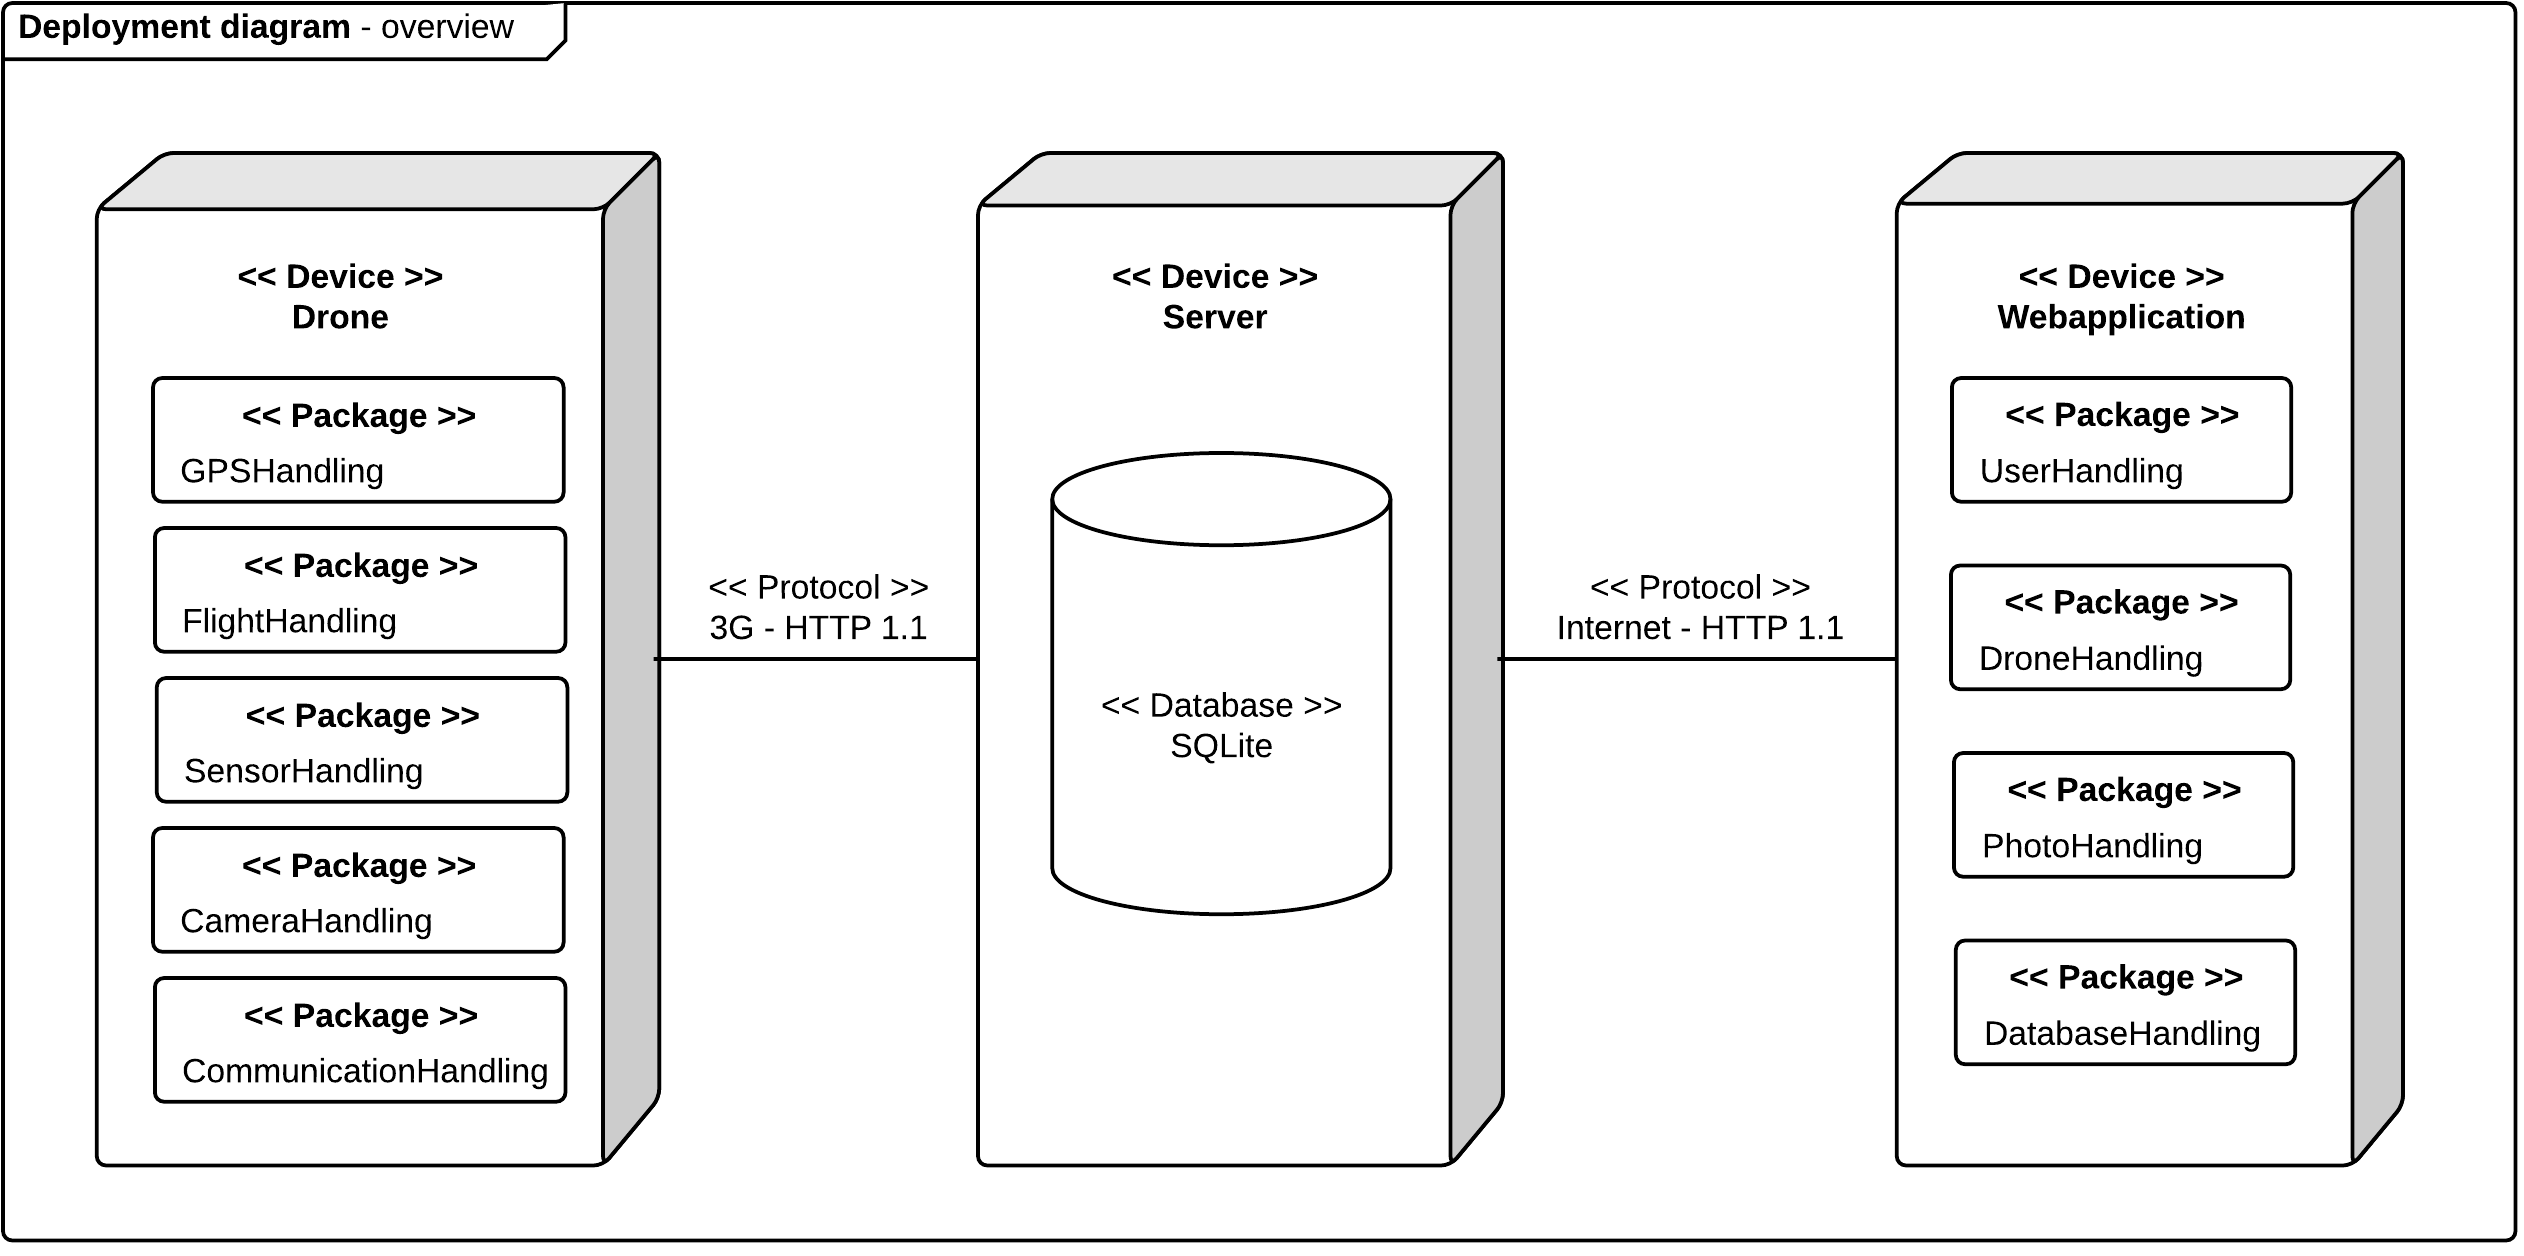
\includegraphics[width=1\textwidth]{Billeder/deployment_overview.png}
\vspace{-0.5cm}
\caption{Deployment diagram}
\label{fig:deployment_diagram}
\end{figure}
 
\newpage


\subsection{Webapplikation}

Webapplikationen fungerer som grænseflade til systemets bruger. Da det ikke ønskes at alle og enhver kan tilgå webapplikationen, skal bruger logge ind før webapplikations funktionalitet kan benyttes. 

Via webapplikationen kan bruger lave nye flyveopsætninger samt monitorere data og information fra tidligere flyvninger. Da det ikke er muligt at rette eller stoppe en aktuel flyvning, skal bruger være opmærksom på hvordan en ny flyveopsætning indstilles. 

Mellem server og webapplikation laves en socket connection. Dette betyder at indholdet af webapplikationen opdateres hver gang der der tilføjes eller ændres i eksisterende data på serverens SQLite database. Yderlige information om webapplikation findes i logical og impelmentation view i \textit{Systemarkitektur og Design} i dokumentationen [xx].


\subsection{HTTP protokol}

Den kommunikationsprotokol der bruges til at sende og modtage data fra server ønskes benyttet af både webapplikation og drone. Da der kun skal laves et interface til server, hvis drone og webapplikation benytter samme protokol.

Webapplikationen kan benytte stort set alle kommunikations protokoller, mens 3G/GPS modulet kun kan benytte et begrænset antal.

Det vælges at benytte HTTP protokollen, da 3G/GPS modulet understøtter denne protokol og fordi protokollen er blandt de mest anvendte protokoller til kommunikation mellem webapplikationer og servere.

Ønskes mere yderlige viden om HTTP protokollen henvises til wikipedia [x] \footnote{http://en.wikipedia.org/wiki/Hypertext\_Transfer\_Protocol} mens der henvis til deployment view i \textit{Systemarkitektur og Design} hvis der ønskes mere viden om brug af protokollen [xx]. 

%%%% Kilder %%%%
\begingroup
\raggedright
\bibliography{bibtex/litteratur}							
% Litteraturlisten inkluderes
\endgroup

%%%% Fixme-listen %%%%
\newpage														% Ny side til Fixme-listen
%\listoffixmes													% Fixme-listen - fjernes til sidst i projektet med "%"

%%%% Appendiks %%%%
\appendix														% Appendiks/bilag start - giver chapter bogstaver i stedet for tal
\clearforchapter												% Sikrer at pagestylen aktiveres paa den rigtige side
\phantomsection													% Kunstigt afsnit, som hyperlinks kan 'holde fast i'
\pdfbookmark[0]{Appendiks}{appendiks}							% Tildeler en klikbar bookmark til den endelige PDF

\end{document}													% Slutter dokumentet - obligatorisk